\documentclass[10pt]{article}
\usepackage[T1]{fontenc}
\usepackage[utf8]{inputenc}
\usepackage{lmodern}
\usepackage[margin=1in]{geometry}
\usepackage{amsmath,amssymb,amsthm,mathtools}
\usepackage{booktabs,longtable,array,tabularx}
\usepackage{graphicx}
\usepackage{xcolor}
\usepackage{microtype}
\usepackage{enumitem}
\usepackage{algorithm}
\usepackage{algpseudocode}
\usepackage[numbers,sort&compress]{natbib}
\usepackage{url}
\usepackage[colorlinks=true,linkcolor=blue!50!black,citecolor=green!40!black,urlcolor=blue!60!black]{hyperref}

\def\UrlBreaks{\do\.\do\_\do\/\do\-}
\DeclareUrlCommand\lean{\urlstyle{tt}}
\newcommand{\lnm}[1]{\lean{VNNUE.#1}}

\newcommand{\Z}{\mathbb{Z}}
\newcommand{\N}{\mathbb{N}}
\newcommand{\R}{\mathbb{R}}
\newcommand{\Zm}[1]{\Z/2^{#1}}
\newcommand{\one}{\mathbf{1}}
\DeclareMathOperator{\supp}{supp}
\DeclareMathOperator{\colops}{colOps}
\DeclareMathOperator{\dec}{dec_{16}}
\DeclareMathOperator{\satop}{sat_{16}}
\DeclareMathOperator{\fold}{fold}
\DeclareMathOperator{\canon}{canon}
\DeclareMathOperator{\clamp}{clamp}
\newcommand{\accV}{\mathrm{acc}^{V}}
\newcommand{\accS}{\mathrm{acc}^{S}}
\newcommand{\psum}{p}
\newcommand{\symd}{\mathbin{\triangle}}

\theoremstyle{plain}
\newtheorem{theorem}{Theorem}[section]
\newtheorem{proposition}[theorem]{Proposition}
\theoremstyle{definition}
\newtheorem{definition}[theorem]{Definition}
\newtheorem{remark}[theorem]{Remark}

\newcommand{\leanref}[1]{\par\smallskip{\raggedright\noindent\upshape\textit{Lean:} #1.\par}}
\newcommand{\hd}[1]{\begin{tabular}[b]{@{}c@{}}#1\end{tabular}}
\Urlmuskip=0mu plus 0.5mu

\title{VNNUE: Very Easily Updatable Neural Networks\\[4pt]
\large An Exact, Formally Verified Update Calculus and a Power-Sum Interaction Channel for Chess Evaluation}
\author{HelloTest006\thanks{Version of 10 November 2026. Lean proofs, experiment code, derived data, result files and the sources of this paper are available at \url{https://github.com/HelloTest006/vnnue} (directories \texttt{lean/}, \texttt{experiments/}, \texttt{paper/}). Code is released under the MIT license; text and figures under CC~BY~4.0.}}
\date{}

\begin{document}
\maketitle

\begin{abstract}
Efficiently updatable neural networks (NNUE) made strong neural evaluation affordable inside alpha-beta chess engines by updating the first layer incrementally on every move.
We revisit this mechanism as an algebraic object.
For a fixed weight table (fixed king bucket and material block), the first layer of an NNUE is a group homomorphism $\Z^N\to(\Zm{16})^L$ from the integer feature-delta group into a lane group.
The \emph{correctness} (not the performance) of incremental updates, Finny-table refreshes, Stockfish's hybrid king update, lazy catch-up and wrap-around integer arithmetic each reduces to an identity of this homomorphism.
We make these identities explicit and machine-checked, and we use the resulting calculus to design VNNUE, a proposed extension of Stockfish's current K32H3 network.

VNNUE adds three things.
The first is a small \emph{power-sum interaction} (PSI) channel.
It is a king-independent, White-absolute accumulator of first and second power sums of a learned embedding, and one copy serves both perspectives.
By the Newton--Girard identities its pre-shift head values equal exact all-pairs piece$\times$piece interaction sums, i.e.\ a factorization machine; the deployed readout then applies a floor shift and clamps.
It costs about $2r$ lanes per changed piece and never needs a refresh.
The second is an exact source-selection policy for accumulator rebuilds whose candidate set contains Stockfish's.
The third is a set of optional modes: low-rank king transitions, net-delta catch-up, and symmetry-equivariant views.

The correctness, range and cost statements are formalized in Lean~4 with Mathlib as 149 theorem declarations in eight modules.
The full build succeeds with no \texttt{sorry}, and the axiom audit of all 149 declarations shows only \texttt{propext}, \texttt{Classical.choice} and \texttt{Quot.sound} (Appendix~\ref{app:lean}).
Formalization also caught several errors in our own draft design (listed in Section~\ref{sec:formal-scope}).

A Python prototype confirms bit-exactness on 6,670,640 accumulator-source checks and 7,803,876 PSI, $y$-state and feature-delta checks with 0 mismatches, on subsets of our data (Section~\ref{sec:e1}).
Under an explicit byte model that charges PSI for its weight columns but not for its own state pass, PSI costs 2.68\% of piece-square column bytes on Lichess games (4.69\% on quiet moves, which meets the proved bound).
The results are mixed elsewhere.
The ``never worse than Stockfish'' source selection, proved under a shared cost model, gains almost nothing beyond taking the minimum over Stockfish's own candidates, and the size of that gain depends on our simulator's cache model.
On lazy toy search traces, greedy net-delta catch-up \emph{increases} whole-trace cost by 20.3\% in columns (9.2\% in FT bytes) relative to the Stockfish-like rule.
The low-rank king transition never wins in the default configuration ($r_K=16$, correction formed on the fly).
PSI learns planted pair structure in small training runs but showed no benefit on real-ish labels.
We make \textbf{no} playing-strength, Elo or speed claim.
VNNUE is a verified architecture proposal, and we list the engine, training and SPRT experiments that would be needed to evaluate it.
\end{abstract}

%=====================================================================
\section{Introduction}
%=====================================================================

The evaluation function of a chess engine is called millions of times per second, at the leaves and interior nodes of an alpha-beta search tree.
Since 2020 Stockfish, the leading open-source engine, has used an \emph{efficiently updatable neural network} (NNUE) for this.
NNUE was introduced for computer shogi by Nasu~\cite{nasu2018} and ported to chess shortly afterwards~\cite{cpwnnue,nnuepytorchdocs}.
The trick is old and simple.
The first layer of the network is a linear map applied to a huge, sparse, binary feature vector.
A move changes only a handful of features, so the first-layer output (the \emph{accumulator}) can be updated by adding and subtracting a few weight columns instead of being recomputed.
This is exactly how engines have always maintained material and piece-square-table scores and Zobrist hash keys~\cite{zobrist1970}.
The only difference is that the scalar or bit-string is replaced by a vector of $L=1024$ int16 lanes.

Over six years the Stockfish community has built many engineering refinements around this core.
King-bucketed feature sets with horizontal mirroring were introduced.
Refresh caches (``Finny tables'')~\cite{sffinny} (an idea the commit credits to Luecx of the Koivisto engine) reconstruct an accumulator from a cached board diff.
A hybrid king-move update combines cached entries~\cite{sfsource}.
Lazy evaluation with catch-up from the last computed ancestor~\cite{sfsource} was added, and two-ply add/remove cancellation~\cite{sfpr5988} followed.
Threat features~\cite{sfthreats} and pawn-pair features came later, and the accumulators use wrapping int16 SIMD arithmetic~\cite{sfsource}.
Each refinement is justified informally and tested by self-play.
None is stated as a theorem.

\paragraph{This paper.}
We take the algebraic view seriously and ask two questions.
First, which statements about NNUE-style accumulators are actually true, under which hypotheses?
Second, can the resulting calculus suggest architecture changes that are ``very easily updatable'', meaning they add expressiveness while keeping the update exact, cheap and refresh-free?
Our answer is VNNUE, a design built on Stockfish's current K32H3 network.
We present it with three kinds of evidence of different strength:
(i)~machine-checked theorems in Lean~4/Mathlib~\cite{demoura2021,mathlib2020};
(ii)~exact operation and byte counts from a Python prototype driven by real game sequences and toy search trees;
(iii)~small training sanity checks.

\paragraph{Contributions.}
\begin{enumerate}[leftmargin=*,itemsep=2pt]
\item \textbf{An exact update calculus for NNUE accumulators} (Section~\ref{sec:theorems}).
For a fixed weight table, accumulators are homomorphisms from the feature-delta group $\Z^N$ into an arbitrary abelian group of lanes.
From this we derive path independence of incremental updates, any-source correctness of refresh caches, the support bound for net deltas, the symmetric-difference metric on cache entries, and exactness of the Stockfish hybrid update.
These are correctness statements; which mechanism is cheaper is a separate, empirical question.
Each statement is instantiated at $\Z$ and at $\Zm{16}$ (wrapping int16 lanes).
\item \textbf{Integer semantics and certificates.}
Wrapping int16 accumulation decodes exactly whenever the \emph{final} value is in range, whatever happens in between.
Saturating arithmetic is provably path-dependent.
Per-lane slot certificates bound lane sums from per-group capacities (the capacities of legal chess positions are an informal input).
We also prove the \texttt{pmaddubsw} pair-safety bound and the quantized-sum rounding bound.
\item \textbf{The PSI channel.}
It is a refresh-free, White-absolute power-sum accumulator that serves both perspectives.
We prove that its pre-shift head values equal a multi-head factorization machine over all piece pairs (T13), that the halving is exact in integers (T12) and the degree-3 power-sum combination is divisible by~6 (T15), that it is incrementally maintainable (T14), and that the exact state and head sums fit in int16/int32 (T9, T16; the int32 head bias and wrapping $\Zm{32}$ semantics are not covered).
It is universal given $N^2$ lanes (T17, an existence result that says nothing about $r=32$), and a PSI lane is not affine (T18d: nonzero mixed second difference, whereas every affine function has zero, T18c); applying T18c to K32H3 PSQ lanes at fixed king and block is an informal step.
\item \textbf{Source selection and optional modes.}
We specify a min-cost source selection whose candidate set strictly contains Stockfish's \{refresh, Finny, hybrid\}, together with its exact never-worse statement and the modelling assumptions it needs.
We also give a low-rank king-transition identity and a symmetry framework based on the Klein four-group acting on 768 features, with 192 orbits.
\item \textbf{A formalization} of 149 theorem declarations (1,907 lines of Lean), all axiom-audited, that compiles against Mathlib v4.35.0 with no \texttt{sorry} (Appendix~\ref{app:lean}).
\item \textbf{An honest experimental report} (Section~\ref{sec:experiments}) that includes several negative results.
\end{enumerate}

\paragraph{Scope and what we do \emph{not} claim.}
VNNUE has not been implemented in a C++ engine, trained at scale, or tested in games.
We make no claim about Elo, playing strength or nodes per second.
Most of our theorems are mathematically easy.
Their value lies in stating the hypotheses exactly (e.g.\ which window a decode is exact on, or which cost function the ``never worse'' guarantee compares), and in the counterexamples that formalization surfaced.
Several of the design's headline hopes did not survive measurement, and we report these in Sections~\ref{sec:experiments} and~\ref{sec:discussion}.

%=====================================================================
\section{Background and a century of history}\label{sec:background}
%=====================================================================

\subsection{Incremental evaluation before NNUE}

Since Shannon~\cite{shannon1950}, chess programs have combined minimax (alpha-beta~\cite{knuth1975}) search with an approximate evaluation function at the leaves.
Two cheap incremental structures became standard in every engine.
The first is the \emph{piece-square table} (PST): the evaluation $\sum_{(p,s)\in\text{pos}}T[p][s]$ is linear in the 768-dimensional one-hot vector of (colour, piece, square), so it updates on a move by $E\gets E-T[p][\mathit{from}]+T[p][\mathit{to}]$.
The second is \emph{Zobrist hashing}~\cite{zobrist1970}: the key $h(\text{pos})=\bigoplus_{f\in\text{pos}}R_f$ is a group homomorphism from feature sets under symmetric difference to $(\Z/2)^{64}$, so it updates by XOR.
Hand-crafted evaluations also contained explicit pairwise terms, for example the quadratic material-imbalance polynomial in piece counts used by pre-NNUE Stockfish~\cite{sf11}, cf. Kaufman's analysis of material imbalances~\cite{kaufman1999}.
Neural evaluation long remained too slow for alpha-beta; AlphaZero~\cite{silver2018} instead paired a large network with Monte Carlo tree search.

\subsection{NNUE and its evolution in Stockfish}

Nasu's NNUE~\cite{nasu2018} reconciled neural evaluation with alpha-beta.
It uses a very wide, sparse, binary input layer (king-relative piece-square features), followed by a small dense network on CPU SIMD integer arithmetic.
The first-layer output is updated incrementally.
NNUE entered Stockfish in August 2020 and shipped in Stockfish~12~\cite{cpwnnue}.
Its subsequent evolution follows our research notes and the cited sources~\cite{nnuepytorchdocs,sfsource,sfreleases}:
\begin{itemize}[leftmargin=*,itemsep=1pt]
\item \emph{Feature sets}: HalfKP, then HalfKA/HalfKAv2, then HalfKAv2\_hm with horizontal mirroring (32 king buckets).
In 2026 these were followed by material-conditioned blocks: K32Q2 (32 own-king buckets $\times$ opponent queen present/absent)~\cite{sfnnv18}, and then K32H3, which has 32 own-king buckets $\times$ 3 material blocks $\times$ 704 piece-squares, giving 67,584 inputs per perspective~\cite{pr563,sfsource}.
\item \emph{Width}: the first layer grew to $L_1=3072$~\cite{pr5149}.
Current master is back at $L_1=1024$ with richer inputs: Full Threats (attacker--target pairs~\cite{sfthreats,sfsource}) and pawn-pair features (PP\_3Wide).
\item \emph{Update machinery}: lazy updates with catch-up from the last computed ancestor~\cite{sfsource}; Finny tables~\cite{sffinny}, which cache per-king-bucket accumulators and rebuild from the board diff; a hybrid update for own-king moves~\cite{sfsource}; two-ply cancellation~\cite{sfpr5988}.
\item \emph{Quantization}: int16 accumulators with non-saturating (wrapping) SIMD adds, int8 hidden weights, a 0..127 activation range (which, as we observe in T10, also keeps \texttt{pmaddubsw} pair sums below $2^{15}$), threat weights stored as int8 and widened to int16~\cite{nnuepytorchdocs,sfsource}, and quantization-aware training in the most recent releases~\cite{sfreleases}.
\end{itemize}
Training is done with nnue-pytorch~\cite{nnuepytorchdocs} or bullet~\cite{bullet}, and changes are accepted by sequential probability ratio tests~\cite{wald1945} on the Fishtest framework~\cite{fishtest}.

\subsection{Mathematical lineage}

VNNUE draws on several well-established lines of mathematics and computer science.

\paragraph{Homomorphisms and finite differencing.}
A linear map $\Phi$ satisfies $\Phi(x+\delta)=\Phi(x)+\Phi(\delta)$.
Incremental maintenance of an expression under small input changes is the subject of Paige and Koenig's \emph{finite differencing}~\cite{paige1982}, of self-adjusting computation~\cite{acar2002}, of change theories for higher-order languages~\cite{cai2014}, and of DBSP's algebra of streams over abelian groups~\cite{budiu2023}.
DBSP's central observation, that linear operators are their own incremental versions and bilinear operators obey a product rule, is exactly what our PSI update rule (Theorem~\ref{thm:t14}) instantiates.
Delta networks~\cite{neil2017} and DeltaCNN~\cite{parger2022} exploit temporal sparsity in deep networks in the same spirit.

\paragraph{Low-rank corrections.}
The Sherman--Morrison--Woodbury identities~\cite{sherman1950,woodbury1950} update a matrix inverse under a low-rank change of the matrix.
We borrow only the base-plus-low-rank-correction pattern, for forward evaluation; our king-transition identity (Theorem~\ref{thm:t23}) is elementary distributivity, in which a rank-$r$ term absorbs the change of king bucket.
Low-rank adaptation~\cite{hu2022lora} is a modern analogue in deep learning.
Closest to C2 is nnue-pytorch's \emph{feature factorization}~\cite{nnuepytorchdocs}: king-bucketed weights are trained as $W_\kappa=R_\kappa+Q$ with a shared ``virtual'' piece-square factor $Q$ that is merged into the bucket weights at export.
C2 restricts the bucket-specific part to rank $r_K$ so that it can be applied incrementally at inference; \lnm{lowrank_generalizes} is the full-rank case of that factorizer.

\paragraph{Power sums and factorization machines.}
The Newton--Girard identities~\cite{macdonald1995} express elementary symmetric polynomials through power sums.
For example $2e_2=p_1^2-p_2$ and $6e_3=p_1^3-3p_1p_2+2p_3$.
Rendle's factorization machines~\cite{rendle2010} use the degree-2 case to compute all pairwise interactions $\sum_{i<j}\langle v_i,v_j\rangle x_ix_j$ in linear time.
Higher-order FMs~\cite{blondel2016} and CP decompositions~\cite{kolda2009} extend the idea.
Sum-of-embeddings pooling $\rho(\sum_x\phi(x))$ is the canonical form of permutation-invariant functions on countable domains~\cite{zaheer2017} (power-sum embeddings appear in their proof for the fixed-size case), and a chess position is a set of pieces.
Pairwise piece interactions are not new in chess evaluation: hand-crafted imbalance tables~\cite{kaufman1999,sf11} are quadratic in piece counts, threat and pawn-pair features are explicit geometric pairs, and Stockfish's FT pairwise product $o_j=u_jv_j$ already forms 512 clipped rank-one quadratic forms per perspective.
What PSI adds is a parametrization: a refresh-free, unclipped, king-independent power-sum state for square-level pair interactions that complements those terms.

\paragraph{Equivariance.}
Group-equivariant networks~\cite{cohen2016} and parameter sharing~\cite{ravanbakhsh2017} tie weights so that a group action on inputs becomes a permutation (a representation) on hidden units.
Stockfish's perspective handling and horizontal mirroring can be viewed as instances of the abstract equivariance statements T21--T22 (Theorems~\ref{thm:t21}--\ref{thm:t22}); the identification with Stockfish's index map is informal.

\paragraph{Integer arithmetic.}
Integer-only inference~\cite{jacob2018} and classical rounding-error analysis~\cite{higham2002} frame our quantization statements.
Roofline thinking~\cite{williams2009} explains why bytes per update, not arithmetic, is the right cost unit for accumulator updates.
Rent-or-buy (ski-rental) competitive analysis~\cite{karlin1988,borodin1998} underlies our appendix lemma on accumulator materialization.

%=====================================================================
\section{The VNNUE architecture}\label{sec:arch}
%=====================================================================

\subsection{Baseline and notation}

\paragraph{Baseline.}
We use Stockfish master as of 9 November 2026, i.e.\ commit \texttt{7cdd5e8} (6 November 2026)~\cite{sfsource}, as the baseline.
Its PSQ feature set is K32H3, with 67,584 inputs per perspective and at most 32 active.
The other feature sets are Full Threats and PP\_3Wide.
The widths are $L_1=1024$, $L_2=32$, $L_3=32$, with 32 layer stacks.
The feature-transformer (FT) output is the pairwise product $o_j=\lfloor\clamp(a_j,0,255)\cdot\clamp(a_{j+512},0,255)/512\rfloor$, giving 512 values per perspective.
The PSQ FT table occupies $67{,}584\times1024\times2$\,B $=138.4$\,MB.
The three blocks (per perspective) are: 0, no rook or queen on the board; 1, some rook or queen, but the opponent has no queen; 2, the opponent has a queen.

\paragraph{Notation.}
We write $[N]=\{0,\dots,N-1\}$ for feature indices and $[L]$ for lanes; in Lean these are \texttt{Fin N} and \texttt{Fin L}.
Let $R$ be an abelian group of lane values: $\Z$ for the specification, $\Zm{16}$ for wrapping int16 lanes.
A weight table is $W:[N]\to R^{L}$, with column $W_i$, and $b\in R^L$ is a bias.
Then
\[
\Phi_W(x)=\sum_{i}x_i\,W_i,\qquad
\accV(b,W,x)=b+\Phi_W(x),\qquad
\accS(b,W,S)=b+\sum_{i\in S}W_i,
\]
for $x\in\Z^N$ and $S\subseteq[N]$.
Here $\one_S$ is the indicator of $S$, $\delta(S,T)=\one_T-\one_S$ is the set delta, $\supp\delta=\{i:\delta_i\neq0\}$, and $\colops(S,T)=|S\symd T|$.
The incremental fold of a list of deltas $\ell=[\delta_1,\dots,\delta_t]$ from an accumulator $a$ is $\fold_W(a,\ell)=(\cdots((a+\Phi_W\delta_1)+\Phi_W\delta_2)\cdots)+\Phi_W\delta_t$.
The absolute feature set is $\mathfrak A=\{0,1\}\times[6]\times[64]$ (colour, piece type, square), with $|\mathfrak A|=768$.
The vector $\beta(\text{pos})\in\{0,1\}^{768}$ is White-absolute and has at most 32 ones.

\paragraph{Cost units.}
\emph{col} is one $L$-wide int16 column add or subtract (2\,KB at $L=1024$).
\emph{mcol} is one $L$-wide multiply-add column, with cost ratio $\mu\geq1$ to col.
\emph{pass} is one accumulator load+store, $2\cdot2L$ bytes.
$k$ is the number of PSQ features changed per perspective: 2 for quiet moves and promotions, 3 for captures, en passant and capture-promotions, 4 for castling.
$k_a$ is the same count in absolute features.
It equals $k$ for every move type, including king moves, because absolute features do not depend on the king.

\subsection{Components}

Table~\ref{tab:components} lists the components.
\textbf{C0} is Stockfish's FT, unchanged.
The headline configuration is C0+C1+C3+C5, with C3 restricted to sources that do not skip materialization (no ancestor net-delta).
\textbf{C4} is \emph{off} by default: the specification enabled it, but its whole-trace effect was negative in our experiments (Section~\ref{sec:e3}), so it awaits a reuse-aware policy.
\textbf{C1$'$}, \textbf{C2}, \textbf{C2$'$} and \textbf{C6} are ablations.

\begin{table}[htbp]
\centering\small
\caption{VNNUE components (state per search-stack ply). ``Default'' marks the headline configuration.}\label{tab:components}
\begin{tabularx}{\linewidth}{@{}lXl@{}}
\toprule
Component & Content & Status\\
\midrule
C0 FT core & $a_c=b+W_{\mathrm{blk}_c,\kappa_c}x_c+W^T\tau_c+W^P\pi_c\in(\Zm{16})^L$, $c\in\{W,B\}$ & unchanged \\
C1 PSI & $P1=V\beta\in(\Zm{16})^r$, $P2=V^{\circ2}\beta\in(\Zm{32})^r$, one copy per position & default \\
C1$'$ PSI deg.~3 & $P1,P2,P3$ for $R$ lanes of $A\in\Z^{R\times768}$, $|A|\le15$ & ablation\\
C2 king transition & $W_{\mathrm{blk},\kappa}=W^0_{\mathrm{blk}}+U_{\mathrm{blk},\kappa}V_K$ (exact in int16; one $V_K$ shared by all blocks); state $y_c=V_Kx_c$ & optional\\
C2$'$ factored king & store $W^0+$region term, $U$, $V_K$; evaluate $a_{\text{base}}+U_\kappa y$ at readout & memory experiment\\
C3 source selection & $\arg\min$ over candidate sources (Table~\ref{tab:sources}) & default\\
C4 net-delta catch-up & $\Delta=\sum_j\delta_j$ with cancellation, one pass & off (negative result)\\
C5 certificates & per-lane slot certificates for C0, C1, C1$'$, C2; checked offline & default\\
C6 symmetry & isotypic threat channel or lane-permutation mirror tying & ablations\\
\bottomrule
\end{tabularx}
\end{table}

\subsection{The PSI channel (C1)}

\paragraph{Parameters and state.}
The parameters are an embedding $V\in\Z^{r\times768}$ (int8, $|V|\le127$), head weights $\Lambda\in\Z^{m\times r}$ (int8), a head bias $b^z\in\Z^m$ (int32) and shifts $\mathit{sh}_e,\mathit{sh}_z$.
The defaults are $r=32$ and $m=16$.
The state is shared between perspectives and White-absolute:
\[
P1_t=\sum_iV_{t,i}\beta_i\ \ (\text{int16}),\qquad P2_t=\sum_iV_{t,i}^2\beta_i\ \ (\text{int32}).
\]
Both are linear in $\beta$, so they update like NNUE columns.
They do not depend on king position or material block, so they \emph{never} need a refresh.

\paragraph{Readout (per evaluation, per perspective).}
\begin{align*}
E_t&=(P1_t^2-P2_t)/2 &&\text{(exact: $2\mid P1_t^2-P2_t$, Thm.~\ref{thm:t12})}\\
\hat e_t&=\clamp(-2^{15},2^{15}-1,\;E_t\gg\mathit{sh}_e)&&\text{(int16)}\\
z_h&=b^z_h+\textstyle\sum_t\Lambda_{h,t}\hat e_t&&\text{(int32; see below)}\\
u_h&=\clamp(0,127,\;z_h\gg\mathit{sh}_z)&&\text{(u8 input to fc\_0, \texttt{pmaddubsw}-safe, Thm.~\ref{thm:t10})}
\end{align*}
For binary $\beta$, $E_t=\sum_{i<j}\beta_i\beta_jV_{t,i}V_{t,j}$, hence
\[
\sum_t\Lambda_{h,t}E_t=\sum_{i<j}\beta_i\beta_jQ^h_{ij},\qquad Q^h=V^\top\mathrm{diag}(\Lambda_h)V
\]
(Theorem~\ref{thm:t13}).
So the pre-shift head value $z_h-b^z_h$ (computed from the exact $E_t$) is a learned sum over \emph{all} ($\le\binom{32}{2}=496$) pairs of present pieces, with a pair table of rank $\le r$ and diagonal core, i.e.\ a multi-head factorization machine~\cite{rendle2010}.
The deployed $u_h$ applies a floor shift, an int16 clamp, a second shift and a 0..127 clamp to it, so it is an FM only approximately.
The shifts and clamps act on the exact state at readout, so they cause no drift over a game; that is a different claim from exactness of the readout.

\emph{Range of $z_h$.} The head sum $\sum_t\Lambda_{h,t}\hat e_t$ is $<2^{31}$ in absolute value for $r\le32$ by Theorem~\ref{thm:t16}(a) (the proof goes through the bound 133,169,152).
The int32 bias $b^z_h$ does not occur in the Lean statement: it must additionally satisfy $|b^z_h|\le2^{31}-1-133{,}169{,}152$, which the export script checks and Lean does not.
Likewise $P2$ is stored as wrapping int32 ($\Zm{32}$), but the Lean development has no $\Zm{32}$ instance and no int32 decode lemma; T9 and T16 bound only the exact integer values of $P1$, $P2$ and $P1^2-P2$.

\paragraph{fc\_0 input and initialization.}
For each layer stack, fc\_0 reads $[o_{\mathrm{stm}};o_{\mathrm{nstm}};u_{\mathrm{stm}};u_{\mathrm{nstm}}]$, which is $1024+2m$ inputs.
Setting the extra fc\_0 columns $B_z=0$ alone makes fc\_0 compute exactly NNUE's $A\,a$, whatever the PSI outputs are (Theorem~\ref{thm:t18}(b)); composing this with the rest of the network into whole-network equality is immediate but not itself formalized.
With $\Lambda=0$ (Theorem~\ref{thm:t18}(a)) the PSI head sums vanish, so $u_h$ is the constant $\clamp(0,127,b^z_h\gg\mathit{sh}_z)$, not $0$ in general.

\paragraph{Perspective sharing without duplication.}
Let $\sigma_c$ be the colour flip $(\mathit{col},\mathit{type},\mathit{sq})\mapsto(1-\mathit{col},\mathit{type},\mathit{sq}\oplus56)$, and let $P$ be an involutive lane permutation.
Because PSI is White-absolute and king-independent, one state serves both perspectives in any case: an untied model can read the same $E$ with perspective-specific heads.
Under the tying constraint $V_{P(t),\sigma_c(i)}=V_{t,i}$, the Black-perspective power sums are moreover the White ones read in permuted lane order: $P1^{(B)}=P1\circ P$ and $P2^{(B)}=P2\circ P$ (Theorem~\ref{thm:t21}).
Tying thus makes the Black readout equal to the White readout under a lane permutation and halves the free parameters of $V$; it does not shrink the state.

\paragraph{Incremental alternative.}
$E$ can be maintained directly.
Adding feature $j$ gives $\Delta E_t=V_{t,j}P1_t(\text{before})$, and removing it gives $\Delta E_t=-V_{t,j}P1_t(\text{after})$ (Theorem~\ref{thm:t14}).
This replaces the $P2$ state by $r$ multiply-adds per changed feature.

\paragraph{What PSI adds, stated correctly.}
It is \emph{false} that NNUE's first layer is affine in $\beta$.
K32H3 is already degree~2 in $\beta$ (king one-hot $\times$ piece-square) and piecewise in material block.
Threat and pawn-pair features are explicit, geometry-gated pairs.
The pairwise product in the FT output creates clipped rank-one quadratics.
The precise statement is narrower: at fixed king squares and fixed block, a K32H3 PSQ lane is affine in the non-king piece indicators, while a PSI lane is not (the PSI half is Theorem~\ref{thm:t18}(d); the K32H3 half is an informal coordinate-wise application of Theorem~\ref{thm:t18}(c)).
PSI therefore adds dense, low-rank, unclipped, king-independent piece$\times$piece terms over all pairs.
They complement the sparse explicit pairs rather than replacing them.
Whether this lowers loss at equal cost is an empirical question (Section~\ref{sec:training}).

\paragraph{Degree 3 (C1$'$, ablation).}
With $A\in\Z^{R\times768}$, $|A|\le15$, state $P1,P2,P3$ per lane, the readout $6e_3=P1^3-3P1\,P2+2P3$ is divisible by 6 (Theorem~\ref{thm:t15}: \lnm{ng3_six_dvd} applied to $y=x\odot v$, which by \lnm{ng3_binary} has the state's power sums for binary $x$; this composition is not a separate Lean lemma).
It is in int32 provided $|P1|\le480$, $|P2|\le7200$, $|P3|\le108{,}000$ (Theorem~\ref{thm:t16}(b)).
These bounds follow from $|A|\le15$ and at most 32 active features by the argument of \lnm{abs_sum_le_card_mul}, but they are not instantiated in Lean.

\subsection{Low-rank king transitions (C2, C2$'$)}

Inside a block, constrain $W_{\mathrm{blk},\kappa}=W^0_{\mathrm{blk}}+U_{\mathrm{blk},\kappa}V_K$.
A single $V_K$ is shared by all blocks and buckets.
The integer factors $U$ (int16) and $V_K$ (int8) are quantized directly, and the stored int16 table is \emph{materialized from the quantized factors}, so the identity holds exactly.
Each perspective maintains $y_c=V_Kx_c\in\Z^{r_K}$.
For an own-king move $\kappa\to\kappa'$ within a block and mirror half (Theorem~\ref{thm:t23}),
\[
a'=a+(U_{\kappa'}-U_\kappa)\,y(\text{before})+W_{\kappa'}(x'-x)\;(+\text{threat/pawn-pair deltas}).
\]
This costs $r_K$ mcol if the difference $\Delta U$ is precomputed or $2r_K$ mcol if it is formed on the fly, plus $k$ col.
A precomputed $\Delta U$ table needs about 18.5\,MB (188 ordered adjacent bucket pairs within a mirror half $\times$ 3 blocks $\times$ $r_K\times L\times2$\,B; up to 25\,MB if 8 neighbours per bucket are assumed) and is not recommended.
The identity is elementary distributivity; we call this source ``Woodbury'' in tables only for the low-rank-correction pattern, not for any matrix inverse.
C2 is one candidate source among several and is \emph{not} claimed to beat Stockfish's hybrid in general.
Like nnue-pytorch's factorizer~\cite{nnuepytorchdocs} it shares a king-independent part across buckets, but it keeps the bucket-specific part low-rank so that it can be applied at inference.
The factored mode C2$'$ stores only the region tables and the factors.
It saves memory (Section~\ref{sec:complexity}) but pays $r_K\cdot L$ multiply-adds per perspective per evaluation: 16,384 MACs per perspective at $r_K=16$, i.e.\ 32,768 for both perspectives, equal to a dense fc\_0 ($1024\times32$).


\subsection{Source selection (C3) and net-delta catch-up (C4)}

When perspective $c$ needs $a=\accS(S)$ in table $T$, any source in Table~\ref{tab:sources} may be used.
A source whose preconditions fail has cost $\top$.
All costs are computable from bitboards and cache metadata before any column is loaded, so the choice is made offline, not as an online (ski-rental) decision.

\begin{table}[htbp]
\centering\small
\caption{Candidate sources for an accumulator build. Stockfish's set is the first three rows.}\label{tab:sources}
\begin{tabularx}{\linewidth}{@{}l>{\raggedright}X>{\raggedright}p{2.3cm}>{\raggedright\arraybackslash}X@{}}
\toprule
id & source & correctness & cost (cols, passes)\\
\midrule
refresh & bias $b$ & definition & $|S|$ col $+\,\tau_{\text{full}}+1$ pass\\
finny & Finny entry with board $C$ & Thm.~\ref{thm:t3} & $|S\symd C|$ col $+1$ pass\\
hybrid & $\mathit{prev}-\mathit{cache}_{\text{old}}+\mathit{cache}_{\text{new}}$ + fix-ups & Thm.~\ref{thm:t24} & $|S_{\text{prev}}\symd C_{\text{old}}|+|S\symd C_{\text{new}}|$ col $+3$ passes (2 extra)\\
woodbury & C2 transition from parent & Thm.~\ref{thm:t23} & $\mu r_K$ (or $2\mu r_K$) $+\,k$ col $+1$ pass\\
ancestor & nearest computed ancestor, net delta & Thms.~\ref{thm:t2},~\ref{thm:t5} & $|\supp\sum_{j>u}\delta_j|$ col $+1$ pass\\
finnyMirror & mirrored Finny entry (C6 tying only) & valid by Thm.~\ref{thm:t21} (over $\Z$; the $\Zm{16}$ version follows via \lnm{castLanes_accV} but is not stated); same cost by Thm.~\ref{thm:t6} & $|S\symd C|$ col $+1$ permutation pass\\
\bottomrule
\end{tabularx}
\end{table}

C4 handles a lazy evaluation at ply $t$ from a materialized ancestor $u$.
It forms $\Delta=\sum_{j=u+1}^t\delta_j$ over sparse index lists, drops zeros, and applies $\Delta$ in one pass.
This generalizes Stockfish's two-ply cancellation~\cite{sfpr5988}.
The author of that change estimated informally (``$\sim$0.2\% I think'') that few three-move updates involve one side moving the same piece twice in a row~\cite{sfpr5988}; this is not a measurement of how many columns cancellation saves.

\subsection{Exact update rules per move type}

Table~\ref{tab:moves} gives the PSI deltas.
King moves are ordinary moves for PSI.
The PSI update is $P1\mathrel{+}=\sum_{f\in A}V_{\cdot,f}-\sum_{f\in R}V_{\cdot,f}$, and likewise for $P2$ with $V^{\circ2}$.
For the FT of perspective $c$ there are five cases.
\begin{enumerate}[leftmargin=*,itemsep=1pt]
\item A non-king move, or an opponent-king move, with the block unchanged: add and subtract columns as in master (if C2 is on, also update $y_c$).
\item An own-king move within the same block and half: C3 over \{refresh, finny, hybrid, woodbury, ancestor\}.
\item An own-king move across the d/e boundary, or castling: C3 over \{refresh, finny, finnyMirror, ancestor\}, with $y_c$ recomputed.
\item A block change: C3 over \{refresh, finny, ancestor\}.
\item A lazy evaluation: chain catch-up from the nearest computed ancestor as in master, or another C3 source if cheaper. C4 (one net-delta pass without materializing intermediates) is an off-by-default option.
\end{enumerate}

\begin{table}[htbp]
\centering\small
\caption{Absolute-feature deltas used by PSI ($c$ = mover, $\bar c$ = opponent).}\label{tab:moves}
\begin{tabular}{@{}llll@{}}
\toprule
Move & removed & added & $k_a$\\
\midrule
quiet (incl.\ non-castling king) & $(c,p,\mathit{from})$ & $(c,p,\mathit{to})$ & 2\\
capture & $(c,p,\mathit{from}),(\bar c,q,\mathit{to})$ & $(c,p,\mathit{to})$ & 3\\
en passant & $(c,P,\mathit{from}),(\bar c,P,\mathit{to}\mp8)$ & $(c,P,\mathit{to})$ & 3\\
promotion to $q$ & $(c,P,\mathit{from})$ & $(c,q,\mathit{to})$ & 2\\
capture-promotion & $(c,P,\mathit{from}),(\bar c,x,\mathit{to})$ & $(c,q,\mathit{to})$ & 3\\
castling & $(c,K,\mathit{ksq}),(c,R,\mathit{rsq})$ & $(c,K,\mathit{ksq}'),(c,R,\mathit{rsq}')$ & 4\\
\bottomrule
\end{tabular}
\end{table}

\begin{algorithm}[htbp]
\caption{VNNUE make/evaluate (specification pseudocode).}\label{alg:vnnue}
\begin{algorithmic}[1]
\Procedure{MakeMove}{$st$, move}
  \State $(R,A)\gets$ absolute delta of move \Comment{Table~\ref{tab:moves}}
  \State $st.P1\gets st.\mathit{parent}.P1+\sum_{f\in A}V_{\cdot f}-\sum_{f\in R}V_{\cdot f}$ \Comment{wrapping int16}
  \State $st.P2\gets st.\mathit{parent}.P2+\sum_{f\in A}V^{\circ2}_{\cdot f}-\sum_{f\in R}V^{\circ2}_{\cdot f}$ \Comment{wrapping int32 (not formalized)}
  \For{$c\in\{W,B\}$} \State record sparse PSQ/threat delta; $st.\mathit{computed}[c]\gets$ false \EndFor
\EndProcedure
\Procedure{Evaluate}{$st$}
  \For{$c\in\{W,B\}$ with $\neg st.\mathit{computed}[c]$}
    \State $s\gets\arg\min_{s\in\textsc{Candidates}(st,c)}\mathit{cost}(s)$ \Comment{C3 (ancestor/C4 off by default)}
    \State $st.\mathit{acc}[c]\gets s.\textsc{Build}()$ \Comment{exact by Thms.~\ref{thm:t2},~\ref{thm:t3},~\ref{thm:t23},~\ref{thm:t24}}
  \EndFor
  \State $o\gets$ pairwise products of $st.\mathit{acc}[\mathrm{stm}],st.\mathit{acc}[\mathrm{nstm}]$ \Comment{as master}
  \State $u\gets(\textsc{PsiReadout}(st,\mathrm{stm}),\textsc{PsiReadout}(st,\mathrm{nstm}))$
  \State \Return $\mathrm{LayerStack}[\mathrm{bucket}(st)](o,u)$
\EndProcedure
\Procedure{PsiReadout}{$st,c$}
  \State $(P1,P2)\gets(st.P1,st.P2)$ if $c=W$ else $(st.P1\circ P,st.P2\circ P)$ \Comment{Thm.~\ref{thm:t21}}
  \State $E\gets(P1^2-P2)\gg1$ \Comment{exact, Thm.~\ref{thm:t12}}
  \State $\hat e\gets\clamp(E\gg\mathit{sh}_e,-32768,32767)$; $z\gets b^z+\Lambda\hat e$ \Comment{$|\Lambda\hat e|<2^{31}$ by T16a; $b^z$ script-checked}
  \State \Return $\clamp(z\gg\mathit{sh}_z,0,127)$
\EndProcedure
\end{algorithmic}
\end{algorithm}

\subsection{Quantization and certificates (C5)}

All accumulators use wrapping arithmetic: $\Zm{16}$ for int16 lanes and $\Zm{32}$ for int32 lanes (the Lean development instantiates only $\Z$ and $\Zm{16}$).

Decoding uses a two's-complement decode $\dec$ with window $[-32768,32767]$.
At export time an offline script checks a per-lane slot certificate (Theorem~\ref{thm:t9}).
Features are grouped (by (colour, type) for PSQ lanes, by square for PSI lanes), and each group gets a legal capacity that allows for promotions: at most 16 pieces per colour, 8 pawns, 10 knights, bishops or rooks, 9 queens, and 1 king.
The certificate then bounds every reachable lane value.
The capacity facts about legal chess positions and the addition of the bias are informal inputs; Lean proves only the implication from per-group caps to the lane-sum bounds (\lnm{slot_certificate}), and the per-colour cap of 16 is not used by that per-group theorem.
Table~\ref{tab:quant} summarizes the types.

\begin{table}[htbp]
\centering\small
\caption{Quantization summary.}\label{tab:quant}
\begin{tabularx}{\linewidth}{@{}>{\raggedright}p{2.6cm}l>{\raggedright}p{3.2cm}>{\raggedright\arraybackslash}X@{}}
\toprule
Tensor & Type & Range & Certificate\\
\midrule
$W_{\mathrm{blk},\kappa}$, $b$ & i16 & as master & Thm.~\ref{thm:t9} per lane\\
$V$ (PSI) & i8 & $|V|\le127$ & $|P1|\le4064$ (i16), $P2\le516{,}128$ (i32)\\
$\Lambda$ & i8 & $|\Lambda|\le127$ & $|\sum_t\Lambda\hat e|<2^{31}$ (Thm.~\ref{thm:t16}a; proof bound 133,169,152)\\
$b^z$ & i32 & -- & $|b^z|+133{,}169{,}152<2^{31}$, script-checked (not in Lean)\\
$A$ (C1$'$) & i8 & $|A|\le15$ & NG3 range given $|P_k|$ bounds (Thm.~\ref{thm:t16}b; bounds not derived in Lean)\\
$U,V_K$ (C2) & i16, i8 & product exactly equals stored i16 table & Thm.~\ref{thm:t9} on materialized table\\
fc\_0 extra columns & i8 & $u_h\in[0,127]$ & \texttt{pmaddubsw} pair bound (Thm.~\ref{thm:t10})\\
\bottomrule
\end{tabularx}
\end{table}

%=====================================================================
\section{The update calculus: theorems}\label{sec:theorems}
%=====================================================================

All statements below are proved in Lean~4 (v4.35.0) against Mathlib (v4.35.0) in namespace \texttt{VNNUE}.
For each one we give the Lean name(s), the statement as the Lean code states it (transcribed into conventional notation), and a short proof idea.
Where the Lean statement is narrower or differs from the design specification, we say so.
Throughout, $R$ is an arbitrary additive commutative group (\texttt{AddCommGroup R}), $W:[N]\to[L]\to R$, $b:[L]\to R$, and $x,\delta\in\Z^N$ act on $R$ by $\Z$-scalar multiplication.
The definitions are those of \texttt{VNNUE/Basic.lean} (Section~\ref{sec:arch}).
Theorem numbers T1--T25 and A1--A2 follow the specification; Appendix~\ref{app:index} gives the complete index.

\subsection{Accumulator algebra (module \texttt{Accumulator})}

\begin{theorem}[T1: homomorphism and delta rule]\label{thm:t1}
For all $W,b,x,y,\delta$:
(a)~$\Phi_W(x+y)=\Phi_W(x)+\Phi_W(y)$;
(b)~$\accV(b,W,x+\delta)=\accV(b,W,x)+\Phi_W(\delta)$;
(c)~$\Phi_W(\delta)=\sum_{i\in\supp\delta}\delta_i\,W_i$.
\leanref{\lnm{Phi_add}, \lnm{accV_add_delta}, \lnm{Phi_eq_sum_supp}; instances \lnm{accV_add_delta_int}, \lnm{accV_add_delta_zmod} at $R=\Z$ and $R=\texttt{ZMod 65536}$}
\end{theorem}
\noindent\emph{Proof idea.} Distribute $\Z$-scalar multiplication over the finite sum; in (c), terms off the support vanish (\texttt{Finset.sum\_filter}).

\begin{theorem}[T2: path independence]\label{thm:t2}
For every list $\ell$ of deltas,
(a)~$\fold_W(\accV(b,W,x),\ell)=\accV(b,W,x+\textstyle\sum\ell)$;
(b)~if $\ell$ is a permutation of $\ell'$, the two folds from $\accV(b,W,x)$ agree;
(c)~for any start $a$ and, for the second identity, $a=\accV(b,W,x)$,
\[\fold_W(a,\ell_1\mathbin{+\!\!+}\ell_2)=\fold_W(\fold_W(a,\ell_1),\ell_2),\qquad \fold_W(a,\ell_1\mathbin{+\!\!+}\ell_2)=\fold_W\big(a,(\textstyle\sum\ell_1)::\ell_2\big),\]
i.e.\ any prefix may be replaced by its net delta.
\leanref{\lnm{foldDeltas_eq}, \lnm{foldDeltas_perm}, \lnm{foldDeltas_append}, \lnm{foldDeltas_group}; instances \lnm{foldDeltas_eq_int}, \lnm{foldDeltas_eq_zmod}}
\end{theorem}
\noindent\emph{Proof idea.} Induction on $\ell$ generalizing $x$, using T1(b); (b) and (c) follow from (a) and \lean{List.Perm.sum_eq} and \lean{List.sum_append}.

\begin{theorem}[T3: set form; any-source correctness]\label{thm:t3}
For finite sets $S,U\subseteq[N]$:
(a)~$\accS(b,W,S)=\accV(b,W,\one_S)$;
(b)~for every $U$,
\[\accS(b,W,S)=\accS(b,W,U)+\sum_{i\in S\setminus U}W_i-\sum_{i\in U\setminus S}W_i;\]
(c)~$\colops(S,U)=|S\setminus U|+|U\setminus S|$;
(d)~$\Phi_W(\delta(U,S))=\sum_{i\in S\setminus U}W_i-\sum_{i\in U\setminus S}W_i$.
Moreover, casting an integer accumulator lane-wise into $\Zm{16}$ equals the accumulator built from the cast bias and cast weights.
\leanref{\lnm{accS_eq_accV}, \lnm{accS_any_source}, \lnm{colOps_eq}, \lnm{Phi_delta}, \lnm{castLanes_accV_int}; instances \lnm{accS_any_source_int}, \lnm{accS_any_source_zmod}}
\end{theorem}
\noindent\emph{Proof idea.} Split each sum over $S$ (resp.\ $U$) into $S\cap U$ and $S\setminus U$ and cancel with \texttt{abel}; (c) is the disjoint union $S\symd U=(S\setminus U)\cup(U\setminus S)$.
Statement (b) is the correctness of every cache-based source: a Finny entry, a stack ancestor, or the empty set (refresh).

\subsection{Delta monoid and cost metric (module \texttt{DeltaMonoid})}

\begin{theorem}[T4: telescoping]\label{thm:t4}
$\delta(S_0,S_1)+\delta(S_1,S_2)=\delta(S_0,S_2)$, $\one_S+\delta(S,T)=\one_T$, and $\supp\delta(S,T)=S\symd T$.
\leanref{\lnm{delta_telescope}, \lnm{ind_add_delta}, \lnm{supp_delta}}
\end{theorem}

\begin{theorem}[T5: net-delta support bound]\label{thm:t5}
$\supp(\delta+\varepsilon)\subseteq\supp\delta\cup\supp\varepsilon$, and for every list $\ell$ of deltas, $|\supp\textstyle\sum\ell|\le\sum_{\delta\in\ell}|\supp\delta|$.
\leanref{\lnm{supp_add_subset}, \lnm{card_supp_sum_le}}
\end{theorem}
\noindent\emph{Proof idea.} Pointwise contrapositive, then induction with \texttt{Finset.card\_union\_le}.
Cancellation can only reduce the number of columns a catch-up touches. It does not follow that greedy catch-up reduces whole-trace cost (Section~\ref{sec:e3}).

\begin{theorem}[T6: $\colops$ is a relabelling-invariant metric]\label{thm:t6}
For finite sets over any type with decidable equality,
$\colops(A,C)\le\colops(A,B)+\colops(B,C)$, $\colops(A,B)=\colops(B,A)$, and for injective $f$, $\colops(f(S),f(C))=\colops(S,C)$.
\leanref{\lnm{colOps_triangle}, \lnm{colOps_comm}, \lnm{colOps_image}}
\end{theorem}
\noindent So routing through an intermediate source never beats the direct diff, and a mirrored cache entry, valid by T21, costs the same (T6).

\subsection{Integer semantics and certificates (module \texttt{Quantization})}

Here $\dec(y)=y.\mathrm{val}$ if $y.\mathrm{val}<32768$ and $y.\mathrm{val}-65536$ otherwise, $\mathrm{InI16}(v)\iff-32768\le v\le32767$, and $\satop(v)=\max(-32768,\min(32767,v))$.

\begin{theorem}[T7: wrap-around exactness]\label{thm:t7}
For integer $b,W,x$ and every list $\ell$ of deltas and lane $j$:
(a)~$\mathrm{cast}(\accV(b,W,x))=\accV(\mathrm{cast}\,b,\mathrm{cast}\,W,x)$ in $(\Zm{16})^L$;
(b)~if $\mathrm{InI16}(v)$ then $\dec((v:\Zm{16}))=v$;
(c)~if $\mathrm{InI16}(\accV(b,W,x+\sum\ell)_j)$ then
\[\dec\big(\fold_{\mathrm{cast}W}(\accV(\mathrm{cast}\,b,\mathrm{cast}\,W,x),\ell)_j\big)=\accV(b,W,x+\textstyle\sum\ell)_j;\]
(d)~Mathlib's $\mathrm{valMinAbs}((v:\Zm{16}))=v$ for $-32768<v\le32768$, and $\mathrm{valMinAbs}((-32768:\Zm{16}))=32768$.
\leanref{\lnm{castLanes_accV}, \lnm{dec16_intCast}, \lnm{wrap_exact}, \lnm{valMinAbs_window}, \lnm{valMinAbs_neg32768}}
\end{theorem}
\noindent\emph{Proof idea.} $\Z\to\Zm{16}$ is a ring homomorphism; (c) is T2 in $\Zm{16}$, then (a), then (b) (by \texttt{ZMod.val\_intCast} and \texttt{omega}).
Only the \emph{final} value needs to be in range; intermediate overflow is irrelevant.
Part (d) records a correction: an earlier draft claimed \texttt{valMinAbs} is exact on $[-2^{15},2^{15})$, which is false at $-2^{15}$.

\begin{theorem}[T8: saturation is path-dependent]\label{thm:t8}
$\satop(\satop(32767+1)+(-1))\neq\satop(32767+\satop(1+(-1)))$, and
$\satop(\satop(30000+30000)+(-30000))=2767$ while $\satop(30000+\satop(30000+(-30000)))=30000$.
\leanref{\lnm{sat16_not_assoc}, \lnm{sat16_path_dependent}}
\end{theorem}
\noindent Saturating adds (\texttt{paddsw}) therefore cannot replace wrapping adds (\texttt{paddw}) in incremental updates. Correctness requires wrapping arithmetic together with a range certificate.

\begin{theorem}[T9: slot certificate and bounds]\label{thm:t9}
Let $g:[N]\to[m]$ be a group map, $w\in\Z^N$ a lane of weights, $M^+_t=\max(0,\max_{g(i)=t}w_i)$ and $M^-_t=\min(0,\min_{g(i)=t}w_i)$ (Lean \texttt{Mplus}, \texttt{Mminus}).
(a)~If $|\{i\in A:g(i)=t\}|\le\mathrm{cap}_t$ for all $t$, then $\sum_t\mathrm{cap}_tM^-_t\le\sum_{i\in A}w_i\le\sum_t\mathrm{cap}_tM^+_t$.
(b)~If $|A|\le K$, $0\le M$ and $w_i\le M$ for all $i$, then $\sum_{i\in A}w_i\le KM$.
(c)~If $|w_i|\le M$ for all $i$, then $|b+\sum_{i\in A}w_i|\le|b|+|A|M$.
(d)~Instances: if $|w_i|\le127$ and $|A|\le32$ then $|\sum_Aw_i|\le4064$ and the sum is in int16 range; if $|w_i|\le127^2$ and $|A|\le32$ then $|\sum_Aw_i|\le516{,}128<2^{31}$.
\leanref{\lnm{slot_certificate}, \lnm{card_bound}, \lnm{global_bound}, \lnm{abs_sum_le_card_mul}, \lnm{P1_bound}, \lnm{P2_bound}, \lnm{P1_numeric}, \lnm{P2_numeric}}
\end{theorem}
\noindent\emph{Proof idea.} Split $A$ into fibres of $g$ (\texttt{Finset.sum\_fiberwise}), bound each fibre by its cardinality times $M^\pm_t$, then by $\mathrm{cap}_t$.
The Lean statement bounds the lane sum without bias. The certified accumulator range adds $b_\ell$.
An earlier ``$\le32$ slots, one active each'' formulation was ill-defined (pieces are unlabelled) and was replaced by this group-map form.

\begin{theorem}[T10: \texttt{pmaddubsw} pair safety]\label{thm:t10}
If $0\le a_1,a_2\le127$ and $|w_1|,|w_2|\le127$, then $|a_1w_1+a_2w_2|\le32258$.
In contrast, $255\cdot127+255\cdot127>32767$.
\leanref{\lnm{pmaddubsw_safe}, \lnm{pmaddubsw_unsafe_255}}
\end{theorem}

\begin{theorem}[T11: quantized-sum rounding error]\label{thm:t11}
Let $s>0$. If $|q_i-sw_i|\le\frac12$ for $i\in A$ and $|q_b-sb|\le\frac12$ (all real), then
$\big|(q_b+\sum_Aq_i)/s-(b+\sum_Aw_i)\big|\le(|A|+1)/(2s)$.
\leanref{\lnm{quant_sum_error}}
\end{theorem}
\noindent Raising the FT scale $s$ shrinks this bound, but it also moves the $0..255$ clamp and the $/512$ product normalization, so it is not a free precision gain.

\subsection{Power-sum interactions (module \texttt{Interaction})}

Write $p_k(v,x)=\sum_ix_iv_i^k$ (Lean \texttt{psum k v x}) and $e_2(y)=\sum_{i<j}y_iy_j$.
Let $e_3^{\mathrm{ord}}(y)$ be the sum of $y_iy_jy_k$ over ordered triples of pairwise distinct indices (so $e_3^{\mathrm{ord}}=6e_3$).
A vector $x$ is binary if every $x_i\in\{0,1\}$.

\begin{theorem}[T12: Newton--Girard order 2 and exact halving]\label{thm:t12}
For every $y\in\Z^N$, $(\sum_iy_i)^2-\sum_iy_i^2=2e_2(y)$.
For binary $x$ and any lane $v$, $p_1(v,x)^2-p_2(v,x)=2e_2(x\odot v)$.
For \emph{every} integer $x$ (binary or not), $2\mid p_1(v,x)^2-p_2(v,x)$.
\leanref{\lnm{ng2}, \lnm{psi_lane}, \lnm{psi_even}}
\end{theorem}
\noindent\emph{Proof idea.} Expand the square as a double sum and split it into $i<j$, $i>j$ and $i=j$. For evenness, write the difference as $2e_2(x\odot v)+\sum_ix_i(x_i-1)v_i^2$, and note that $x(x-1)$ is even.

\begin{theorem}[T13: PSI heads are an all-pairs factorization machine]\label{thm:t13}
For $V\in\Z^{r\times N}$, $\Lambda\in\Z^{m\times r}$, binary $x$ and every head $h$,
\[
\sum_t\Lambda_{h,t}\big(p_1(V_t,x)^2-p_2(V_t,x)\big)=2\sum_{i<j}x_ix_j\sum_t\Lambda_{h,t}V_{t,i}V_{t,j}.
\]
\leanref{\lnm{psi_heads}}
\end{theorem}

\begin{theorem}[T14: incremental rules]\label{thm:t14}
For all integer $x,\delta$ and every feature $j$ (with $e_j$ the unit vector):
$p_k(v,x+\delta)=p_k(v,x)+p_k(v,\delta)$;
\[
q(x+e_j)=q(x)+2v_j\,p_1(v,x),\qquad q(x-e_j)=q(x)-2v_j\,p_1(v,x-e_j),
\]
where $q(x)=p_1(v,x)^2-p_2(v,x)$.
\leanref{\lnm{psum_add}, \lnm{psi_add_feature}, \lnm{psi_remove_feature} (helper \lnm{psum_single})}
\end{theorem}
\noindent This is the DBSP-style product rule~\cite{budiu2023}: $\Delta E=v_jP1(\text{before})$ on add and $-v_jP1(\text{after})$ on remove. No binarity hypothesis is needed.

\begin{theorem}[T15: Newton--Girard order 3 and divisibility by 6]\label{thm:t15}
For every $y\in\Z^N$, $e_3^{\mathrm{ord}}(y)=p_1^3-3p_1p_2+2p_3$ with $p_k=\sum_iy_i^k$, and $6\mid p_1^3-3p_1p_2+2p_3$.
For binary $x$, $e_3^{\mathrm{ord}}(x\odot v)=p_1(v,x)^3-3p_1(v,x)p_2(v,x)+2p_3(v,x)$.
\leanref{\lnm{ng3}, \lnm{ng3_six_dvd}, \lnm{ng3_binary}}
\end{theorem}
\noindent\emph{Proof idea.} Inclusion--exclusion over the diagonals $\{i=j\},\{j=k\},\{i=k\}$ of the triple sum. Divisibility by 2 follows from T12, and divisibility by 3 from $(\sum y)^3\equiv\sum y^3\pmod 3$ (proved by induction on the index set); then use $\gcd(2,3)=1$.

\begin{theorem}[T16: int32 range certificates]\label{thm:t16}
(a)~If $r\le32$, $|\Lambda_t|\le127$ and $|e_t|\le32768$, then $|\sum_t\Lambda_te_t|<2^{31}$ (the proof goes through the bound $32\cdot127\cdot32768=133{,}169{,}152$).
(b)~If $|p_1|\le480$, $|p_2|\le7200$, $|p_3|\le108{,}000$, then $|p_1^3-3p_1p_2+2p_3|<2^{31}$.
(c)~If $|P1|\le4064$ and $0\le P2\le516{,}128$, then $|P1^2-P2|<2^{31}$.
\leanref{\lnm{mix_range}, \lnm{ng3_range}, \lnm{e_lane_range}}
\end{theorem}
\noindent An earlier version of (b) assumed only a bound on $p_1$ and was false (take $p_1=0$, $p_3=2^{31}$). The Lean statement carries all three hypotheses.

\begin{theorem}[T17: universality given $N^2$ lanes]\label{thm:t17}
For every integer pair table $Q\in\Z^{N\times N}$ there exist $r$, $V\in\Z^{r\times N}$ and $\lambda\in\Z^r$ such that for every binary $x$,
$\sum_t\lambda_t(p_1(V_t,x)^2-p_2(V_t,x))=2\sum_{i<j}Q_{ij}x_ix_j$.
\leanref{\lnm{psi_universal} (helpers \lnm{psum_pair}, \lnm{lane_pair}, \lnm{pair_sum})}
\end{theorem}
\noindent The construction uses $r=N^2$ lanes indexed by ordered pairs $(a,b)$, pair lanes $V=e_a+e_b$, and $\lambda=Q_{ab}$ if $a<b$, else $0$. The specification proposed $r=\binom N2$; the Lean witness is wasteful but simpler. An earlier claim that ``$V=I$ gives every diagonal-core table'' is false ($V=I$ gives $z\equiv0$).
T17 is an existence statement at $r=N^2$ and says nothing about the deployed $r=32$.

\begin{theorem}[T18: strict generalization and non-affinity]\label{thm:t18}
(a)~With $\Lambda=0$, the head sum $\sum_t\Lambda_{h,t}(p_1(V_t,x)^2-p_2(V_t,x))$ is $0$ for every $V,x$ (before bias, shift and clamp).
(b)~If the extra fc\_0 block $B_z=0$, then $A\,a+B_z z=A\,a$.
(c)~For every $f(x)=c+w_0x_0+w_1x_1$ on two indicators, $f(1,1)-f(1,0)-f(0,1)+f(0,0)=0$.
(d)~For the lane $v=(1,1)$ and $q(x)=p_1(v,x)^2-p_2(v,x)$, $q(1,1)-q(1,0)-q(0,1)+q(0,0)=2$.
\leanref{\lnm{psi_zero_heads}, \lnm{fc0_embed}, \lnm{affine_second_diff}, \lnm{psi_not_affine}}
\end{theorem}
\noindent Part (b) shows that with the extra fc\_0 columns $B_z=0$, fc\_0 computes exactly NNUE's $A\,a$, whatever the PSI outputs are. Part (a) shows that at $\Lambda=0$ the PSI input is a constant ($b^z$ after shift and clamp). Composing these into whole-network equality (layer stacks, clipping) is immediate but not itself formalized.
Parts (c)--(d) support the claim that PSI lanes are not affine in piece indicators.
The application to K32H3 (``at fixed king squares and block, a PSQ lane is affine in the non-king piece indicators'') is an informal coordinate-wise use of (c) and is not itself a Lean statement.

\subsection{Symmetry (module \texttt{Symmetry})}

Squares are $[64]$; $\mathrm{mirH}(s)$ maps file $f\mapsto7-f$ ($s\oplus7$) and $\mathrm{flipV}(s)$ maps rank $\rho\mapsto7-\rho$ ($s\oplus56$).
Features are $\mathfrak A=[2]\times[6]\times[64]$, with $\sigma_h(c,p,s)=(c,p,\mathrm{mirH}\,s)$, $\sigma_c(c,p,s)=(1-c,p,\mathrm{flipV}\,s)$, and $\canon(i)$ which first normalizes the colour to $0$ (applying $\sigma_c$ if needed) and then the file to e--h (applying $\sigma_h$ if needed).

\begin{theorem}[T19: Klein four-group on squares]\label{thm:t19}
$\mathrm{mirH}$ and $\mathrm{flipV}$ are commuting involutions, and $\mathrm{mirH}$, $\mathrm{flipV}$ and $\mathrm{mirH}\circ\mathrm{flipV}$ have no fixed squares.
Exactly 32 squares lie on files e--h, and $\mathrm{mirH}$ maps the a--d squares onto the e--h squares (and e--h into a--d).
\leanref{\lnm{klein_squares}, \lnm{king_half}, \lnm{king_half_onto}}
\end{theorem}

\begin{theorem}[T20: free action and 192 orbits]\label{thm:t20}
For every $i\in\mathfrak A$: $\sigma_hi\neq i$, $\sigma_ci\neq i$, $\sigma_h\sigma_ci\neq i$.
$\canon$ is invariant under $\sigma_h$ and $\sigma_c$, lands in colour 0 and files e--h, fixes such features, and $\canon(i)\in\{i,\sigma_hi,\sigma_ci,\sigma_h\sigma_ci\}$.
Furthermore $\canon i=\canon k\iff k\in\{i,\sigma_hi,\sigma_ci,\sigma_h\sigma_ci\}$, and $|\canon(\mathfrak A)|=192$.
\leanref{\lnm{feat_free}, \lnm{canon_invariant}, \lnm{canon_mem}, \lnm{canon_fix}, \lnm{canon_mem_orbit}, \lnm{canon_eq_iff}, \lnm{canon_image_card}}
\end{theorem}
\noindent Hence the free Klein-group action has exactly $768/4=192$ orbits, and full tying leaves 192 free columns. The proofs avoid \texttt{native\_decide}, so the trusted base is not enlarged.

\begin{theorem}[T21: equivariance and PSI perspective sharing]\label{thm:t21}
Let $\sigma\in\mathrm{Perm}([n])$ and $\pi\in\mathrm{Perm}([L])$, with integer $W$ tied by $W_{\sigma i}(\pi j)=W_i(j)$.
Then $\sum_ix_{\sigma^{-1}i}W_i(\pi j)=\sum_ix_iW_i(j)$. If moreover $b(\pi j)=b(j)$, then $\accV(b,W,x\circ\sigma^{-1})(\pi j)=\accV(b,W,x)(j)$.
For PSI, if $V_{P t}(\sigma i)=V_t(i)$, then $p_k(V_{Pt},x\circ\sigma^{-1})=p_k(V_t,x)$ for $k=1,2$.
For the concrete colour flip $\sigma_c$ on $\mathfrak A$ and every $k$: if $V_{Pt}(\sigma_ci)=V_t(i)$ then $\sum_ix_{\sigma_ci}V_{Pt}(i)^k=\sum_ix_iV_t(i)^k$.
\leanref{\lnm{acc_equivariant}, \lnm{acc_equivariant_accV}, \lnm{psi_shared}, \lnm{psi_shared_sigC}}
\end{theorem}
\noindent\emph{Proof idea.} Reindex the sum by $\sigma$ (\texttt{Equiv.sum\_comp}) and rewrite with the tying hypothesis.

\begin{theorem}[T22: regular representation and isotypic split]\label{thm:t22}
Let $\sigma$ be an involution on $[n]$ and $W'_i=(W_i,W_{\sigma i})$ on lanes $[L]\sqcup[L]$.
Then $W'_{\sigma i}(k)=W'_i(\mathrm{swap}\,k)$, and $\sum_ix_iW'_i(\mathrm{inr}\,j)=\sum_ix_{\sigma i}W_i(j)$.
For $u,v\in\Z^L$: $(u+v)+(u-v)=2u$ and $(u+v)-(u-v)=2v$.
With $a_\pm(x)_j=\sum_ix_i(W_i(j)\pm W_{\sigma i}(j))$ we have $a_+(x\circ\sigma)=a_+(x)$ and $a_-(x\circ\sigma)=-a_-(x)$.
The map $(u,v)\mapsto(u+v,u-v)$ is injective on $\Z^L\times\Z^L$, but there are no integers with $u+v=1$, $u-v=0$.
\leanref{\lnm{regular_rep}, \lnm{isotypic}, \lnm{isotypic_action}, \lnm{isotypic_inj}, \lnm{isotypic_not_surj}}
\end{theorem}
\noindent Stockfish's horizontal-mirror canonicalization is the regular-representation case. The isotypic split makes a mirror crossing cost \emph{one negation pass} over $a_-$ (not ``no arithmetic'', as an earlier draft said), at the price of factor-2 scales because the change of basis is not unimodular.

\subsection{Refresh and source selection (module \texttt{Refresh})}

\begin{theorem}[T23: low-rank king transition]\label{thm:t23}
Over any commutative ring $S$, for $W^0\in S^{L\times n}$, $U,U'\in S^{L\times r}$, $V\in S^{r\times n}$ and $x,x'\in S^n$:
\begin{align*}
(W^0+U'V)x'&=(W^0+UV)x+(W^0+U'V)(x'-x)+(U'-U)(Vx),\\
Vx+V(x'-x)&=Vx',\qquad (W^0+UV)x=W^0x+U(Vx).
\end{align*}
(Every family $W_k$ equals $0+W_k\cdot I$, i.e.\ the factorization at inner dimension $r=n$ is trivially general.)
\emph{However}, over any field $F$, if $r<n$ there is no $W^0$, $V\in F^{r\times n}$, $U_0,U_1$ with $W^0+U_0V=0$ and $W^0+U_1V=I_n$. Concretely, this fails over $\mathbb Q$ with $n=2$, $r=1$.
\leanref{\lnm{king_transition}, \lnm{king_transition_y_update}, \lnm{factored_eq_merged}, \lnm{lowrank_generalizes}, \lnm{lowrank_proper}, \lnm{lowrank_proper_rat_2_1}; instances \lnm{king_transition_int}, \lnm{king_transition_zmod}, \lnm{factored_eq_merged_int}, \lnm{factored_eq_merged_zmod}}
\end{theorem}
\noindent\emph{Proof idea.} Matrix--vector distributivity and \texttt{abel}. For \texttt{lowrank\_proper}, $(U_1-U_0)V=I_n$ would have rank $\le r<n$.
\begin{remark}[Correction]
The design specification presented \texttt{lowrank\_generalizes} as showing that low-rank king conditioning ``generalizes'' independent buckets.
That is true only at full inner dimension $r=n$.
\texttt{lowrank\_proper} (stated for square $L=n$ tables over any field) shows that for $r<n$ the factored family cannot represent even $\{0,I_n\}$.
The same obstruction applies to the deployed $1024\times704$ tables at $r_K=16$ by zero-padding and viewing integer weights over $\mathbb Q$; that extension is an informal corollary, not a separate Lean theorem.
So the expressiveness-preservation reading of \texttt{lowrank\_generalizes} is wrong.
The cost of the restriction is an empirical question (Section~\ref{sec:e5}).
The identity also covers only transitions with a shared $W^0$, i.e.\ within one block and region. Block changes go through refresh or Finny.
\end{remark}

\begin{theorem}[T24: source selection never worse; hybrid correct]\label{thm:t24}
Let $\mathrm{Src}$ be the six sources refresh, finny, hybrid, woodbury, ancestor and finnyMirror, and let $\mathrm{SF}=\{\text{refresh},\text{finny},\text{hybrid}\}\subseteq\mathrm{Src}$.
(a)~For finite $C_1\subseteq C_2$ with $C_1\neq\emptyset$ and any $f$ into a linear order, $\min_{C_2}f\le\min_{C_1}f$.
In particular, for every $\mathrm{cost}:\mathrm{Src}\to\N\cup\{\top\}$ (or into any linear order), $\min_{\mathrm{Src}}\mathrm{cost}\le\min_{\mathrm{SF}}\mathrm{cost}$.
With two cost functions, if $\mathrm{cost}_V(s)\le\mathrm{cost}_{SF}(s)$ for $s\in\mathrm{SF}$, then $\min_{\mathrm{Src}}\mathrm{cost}_V\le\min_{\mathrm{SF}}\mathrm{cost}_{SF}$.
(b)~For all $b,W,W',S,S_{\text{prev}},C_{\text{old}},C_{\text{new}},T,T'$:
\begin{multline*}
\accS(b,W',S)+T'=(\accS(b,W,S_{\text{prev}})+T)
-\big(\accS(b,W,C_{\text{old}})+\textstyle\sum_{S_{\text{prev}}\setminus C_{\text{old}}}W-\sum_{C_{\text{old}}\setminus S_{\text{prev}}}W\big)\\
+\big(\accS(b,W',C_{\text{new}})+\textstyle\sum_{S\setminus C_{\text{new}}}W'-\sum_{C_{\text{new}}\setminus S}W'\big)+(T'-T),
\end{multline*}
together with the same identity in Stockfish's implementation order (fix-ups applied to $\mathit{prev}-\mathit{cache}_{\text{old}}+\mathit{cache}_{\text{new}}$ in one pass), and its instance at $\Zm{16}$.
\leanref{\lnm{inf'_superset}, \lnm{never_worse}, \lnm{never_worse_general}, \lnm{never_worse_dominated}, \lnm{hybrid_correct}, \lnm{hybrid_correct_impl}, \lnm{hybrid_correct_zmod}, \lnm{refresh_accS_any_source}}
\end{theorem}
\noindent The never-worse statement is pure monotonicity of the minimum, and its content lies entirely in its \emph{modelling assumptions}, which the Lean docstrings make explicit.
(i)~Either one cost function is shared by both engines, or per-source dominance holds (\texttt{never\_worse\_dominated}). Neither is automatic, because VNNUE may use merged or factored tables, pays the C2$'$ readout tax, and may hold different cache contents.
(ii)~The overhead of computing the candidate costs is excluded.
(iii)~Only the FT-column part is covered, and PSI adds its own term (T25).
The specification's \texttt{deriving Fintype} for $\mathrm{Src}$ does not elaborate in this toolchain, so the Lean development lists the six constructors by hand and checks $|\mathrm{Src}|=6$ by \texttt{decide}. No statement is affected.

\subsection{Complexity (module \texttt{Complexity})}

\begin{theorem}[T25: PSI overhead and king-event total]\label{thm:t25}
For naturals $k,L,e,\mathrm{cost}_N$ with $4kL\le\mathrm{cost}_N$:
(a)~$4L(\mathrm{cost}_N+ke)\le(4L+e)\,\mathrm{cost}_N$; if $L>0$, then $ke/\mathrm{cost}_N\le e/(4L)$ as reals;
with $e=192$, $L=1024$: $1000(\mathrm{cost}_N+192k)\le1047\,\mathrm{cost}_N$, i.e.\ at most 4.7\% (exactly $192/4096=4.6875\%$).
(b)~For candidate sets $C_1\subseteq C_2$ with $C_1$ nonempty and any $f:\iota\to\N$, $\min_{C_2}f+ke\le\min_{C_1}f+ke$.
\leanref{\lnm{psi_overhead}, \lnm{psi_overhead_ratio}, \lnm{psi_overhead_instance}, \lnm{psi_overhead_instance_exact}, \lnm{king_event_total} (helper \lnm{inf'_superset_cx})}
\end{theorem}
\noindent The hypothesis $4kL\le\mathrm{cost}_N$ says that NNUE streams at least $k$ columns per perspective for both perspectives.
Here $e$ is a modelling choice: the bytes of PSI traffic charged per changed absolute feature.
We use $e=6r$ (the widths of the $r$ int16 lanes of $P1$ and $r$ int32 lanes of $P2$, $2r+4r$ bytes), so $r=32$ gives $e=192$; if $V$ is stored as int8 and $V^{\circ2}$ as int16, the weight columns are only $3r$ bytes, so $6r$ is conservative for column traffic.
T25 compares only against NNUE's \emph{column} bytes.
It says nothing about ratios that include accumulator passes: those must also charge PSI its own state pass (load and store of $P1,P2$, $2\cdot6r=12r=384$\,B per make), which our E2 byte model omits (Section~\ref{sec:e2}).

\begin{theorem}[A1: ski-rental materialization]\label{thm:a1}
Let $\mathrm{alg}(B,n)=n$ if $n<B$, else $2B-1$, and $\mathrm{algT}(B,t,n)=n$ if $n\le t$, else $t+B$. For $B\ge1$: $B\cdot\mathrm{alg}(B,n)\le(2B-1)\min(n,B)$ for every $n$, and for every threshold $t$, $(2B-1)\min(t+1,B)\le B\cdot\mathrm{algT}(B,t,t+1)$.
\leanref{\lnm{ski_upper}, \lnm{ski_lower}}
\end{theorem}
\noindent This is the classical rent-or-buy (ski-rental) bound~\cite{karlin1988}, in its discrete $(2-1/B)$ form~\cite{borodin1998}, applied to the only genuinely online decision: whether to materialize an intermediate accumulator.

\begin{theorem}[A2: fused-pass traffic]\label{thm:a2}
For per-ply column counts $ks$ (length $t\ge1$), $k_{\text{net}}\le\sum ks$, column cost $c$ and pass cost $2a$:
$k_{\text{net}}c+2a+2a(t-1)\le\sum_j(k_jc+2a)$, and therefore $k_{\text{net}}c+2a\le\sum_j(k_jc+2a)$.
\leanref{\lnm{fused_traffic}, \lnm{fused_one_pass} (helper \lnm{sum_map_traffic_cx})}
\end{theorem}

\subsection{What the formalization did and did not establish}\label{sec:formal-scope}

The formalization covers the \emph{algebra} of updates and range arguments over abstract index sets.
It does not model chess move generation, the K32H3 index map, the threat feature set, SIMD code, or Python or C++ implementations.
The link between theorems and code is the empirical bit-exactness test E1 (Section~\ref{sec:e1}).
During design and formalization, several statements in earlier drafts were found to be false and were corrected. The Lean versions encode the corrections, and several of the counterexamples are themselves theorems:
the \texttt{valMinAbs} window (T7d),
the degree-3 range lacking $p_2,p_3$ hypotheses (T16b),
``$V=I$ gives every diagonal-core table'' (replaced by T17),
``NNUE's first layer is affine in $\beta$'' (restated as T18c/d),
``never worse than Stockfish'' with Stockfish's set lacking hybrid (T24 includes hybrid),
the isotypic ``no arithmetic'' claim (T22: one negation pass),
and the expressiveness reading of low-rank king buckets (T23, \texttt{lowrank\_proper}).
These were errors in our own specification, caught before implementation; they are not findings about NNUE or Stockfish.
Several PSI-related links are also informal: the int32 bias $b^z$ and the $\Zm{32}$ wrapping of $P2$ (Section~\ref{sec:arch}), the degree-3 divisibility for the binary-weighted state and the $|P_k|$ hypotheses of T16(b), and the composition of T18(a)--(b) into whole-network equality.


%=====================================================================
\section{Complexity and memory analysis}\label{sec:complexity}
%=====================================================================

This section is analytic. It uses the specification's cost model ($L=1024$; 1 col = 2\,KB; $e=6r$ bytes, i.e.\ $2r$ lanes, of PSI traffic per changed absolute feature) and is not measured.
The PSI charge $e$ covers PSI's weight columns; PSI's own state pass (load and store of $P1,P2$, $12r=384$\,B per make) is not part of $e$ and is discussed in Section~\ref{sec:e2}.
Section~\ref{sec:experiments} measures the same quantities on real move sequences.

\begin{table}[htbp]
\centering\small
\caption{Per-move update cost, both perspectives (analytic). $\tau_c,\pi_c$: changed threat and pawn-pair features; $d_F=|S\symd C_{\text{new}}|$, $d_{\text{old}}=|S_{\text{prev}}\symd C_{\text{old}}|$; defaults $r=32$, $m=16$.}\label{tab:cost}
\begin{tabularx}{\linewidth}{@{}>{\raggedright}p{3.3cm}>{\raggedright}X>{\raggedright}X>{\raggedright\arraybackslash}p{2.7cm}@{}}
\toprule
Move type & NNUE (master) & VNNUE (default) & PSI extra (shared)\\
\midrule
Quiet non-king ($k=2$) & $2k+\sum_c(\tau_c+\pi_c)$ col & same & 128 lanes (384\,B)\\
Capture / e.p.\ / cap.-promo ($k=3$) & $2k+\sum_c(\tau_c+\pi_c)$ col & same & 192 lanes (576\,B)\\
Promotion ($k=2$) & $2k+\sum_c(\tau_c+\pi_c)$ col & same & 128 lanes\\
Own king, same block and half & $\min(|S|+\tau_{\text{full}},\,d_F,\,d_{\text{old}}+d_F+2\,\text{pass})$ + other side $k$ & min over the superset (adds $\mu r_K+k+\tau$ and ancestor) + other side $k$ & $k\cdot2r$ lanes\\
Own king across d/e, castling & $\min(|S|+\tau_{\text{full}},d_F)$ + other side & $\min(\dots,\text{finnyMirror if C6})$ + other side & $k\cdot2r$ lanes\\
Block change & refresh/Finny both sides & same (C3 superset) & $k\cdot2r$ lanes\\
$t$-ply lazy catch-up & $\sum_jk_j$ col + about $t$ passes & $|\supp\sum_j\delta_j|$ col + 1 pass & $\sum_jk_j\cdot2r$ lanes (eager)\\
\midrule
Per evaluation & pairwise 1024 products; fc\_0 $\le32{,}768$ MACs & same & $2\cdot512+1024=2048$ MACs\\
Per evaluation, C2$'$ & -- & $+\,r_KL$ MACs per perspective (32,768 for both at $r_K=16$) & \\
\bottomrule
\end{tabularx}
\end{table}

Table~\ref{tab:cost} gives the per-move costs.
Two statements are proved.
First, per build event, from identical accumulator and cache state and under a shared cost function (the T24 assumptions), VNNUE's FT column cost is $\le$ the minimum over Stockfish's candidates.
This does not compose over a search: see E3 (Section~\ref{sec:e3}), where greedy C4 raises whole-trace columns by 20.3\% on lazy trees.
Second, PSI's weight-column traffic is at most $e/(4L)=4.6875\%$ of NNUE's PSQ column traffic whenever NNUE streams at least $k$ columns per perspective (T25).
The bound is tight for quiet moves.
The ratio falls once NNUE's passes and threat churn (``3--4$\times$ as many changing threat features as piece features in a typical midgame''~\cite{nnuepytorchdocs}) are included, but such ratios must also charge PSI its state pass.
Non-king moves therefore do strictly \emph{more} work in VNNUE.
King moves are never worse in column count per event, under the T24 cost assumptions.
Wall-clock effects depend on cache residency: the 24\,KB $V$ table, plus 48\,KB if $V^{\circ2}$ is stored, should stay in L1/L2, whereas FT columns stream from L3 or DRAM.
We have not measured this.

The per-evaluation PSI readout costs 2048 multiply-adds at $r=32$, $m=16$.
That is 6.3\% of a dense fc\_0, and a larger share of Stockfish's sparse fc\_0.
The factored C2$'$ mode costs $r_KL$ MACs per perspective per evaluation.
At $r_K=16$ this is 16,384 MACs per perspective, i.e.\ 32,768 for both perspectives, equal to a dense fc\_0 ($1024\times32$): a real tax that has to be bought back by memory savings.

\begin{table}[htbp]
\centering\small
\caption{Memory (analytic). $|P|$: number of king regions in C2$'$. Units: MB $=10^6$\,B, KB $=1024$\,B.}\label{tab:memory}
\begin{tabularx}{\linewidth}{@{}>{\raggedright}p{3.0cm}>{\raggedright}p{2.6cm}>{\raggedright}p{2.2cm}>{\raggedright}X>{\raggedright\arraybackslash}X@{}}
\toprule
Item & NNUE master & VNNUE default & + C2 merged ($r_K=16$) & + C2$'$ factored ($|P|=4$, $r_K=16$)\\
\midrule
PSQ FT table & $67{,}584\times1024\times2$\,B $=138.4$\,MB & 138.4\,MB & 138.4\,MB + $U$: 3.1\,MB + $V_K$: 11\,KB & $3\cdot4\cdot704\cdot1024\cdot2$\,B $=17.3$\,MB + 3.1\,MB $=20.4$\,MB\\
PSI $V$ / $V^{\circ2}$ & -- & 24\,KB / 48\,KB & same & same\\
$\Lambda$, $b^z$ & -- & 512\,B + 64\,B & same & same\\
fc\_0 extra & -- & 32\,KB & same & same\\
Per-ply state & $2\times2$\,KB + threat state & + 64\,B ($P1$) + 128\,B ($P2$), once per position & + $2\times32$\,B ($y$) & same\\
Finny entry & acc + board & unchanged & + $y$ (32\,B) & + $y$\\
\bottomrule
\end{tabularx}
\end{table}

Table~\ref{tab:memory} gives the memory footprint.
The only large potential saving is C2$'$, which would make the PSQ table about 6.8 times smaller.
It pays the readout tax above, and E5 (Section~\ref{sec:e5}) shows that the integer-factor constraint is costly without quantization-aware training.

%=====================================================================
\section{Experiments}\label{sec:experiments}
%=====================================================================

\paragraph{Setup and scope.}
All numbers in this section are copied from \texttt{experiments/RESULTS.md}, which is generated mechanically from \texttt{experiments/results/*.json}.
The machine was a 4-core Windows laptop CPU with Python 3.14, numpy 2.4, torch 2.10 (CPU) and python-chess 1.11, and all seeds were fixed.
This is a Python prototype.
Op and byte counts are exact counts under an explicit cost model.
Wall-clock numbers are numpy/torch proxies that do not represent SIMD C++.
The search traces come from a toy alpha-beta searcher, not from Stockfish.
\textbf{No statement in this section concerns playing strength, Elo or nps.}

\paragraph{Pre-registered hypotheses.}
The design specification stated three hypotheses before the experiments, which are our own priors:
H1, PSI byte overhead $\le4.7\%$ of PSQ column traffic (the T25 bound) under the byte model;
H2, at $r_K=16$ with $\Delta U$ formed on the fly, the low-rank (``Woodbury'') source wins fewer than 10\% of own-king events;
H3, C4's column saving from cancellation is $<1\%$.

\paragraph{Data.}
We used three sources (Table~\ref{tab:data}).
The first is the first 3,000 standard games from the January 2013 Lichess database~\cite{lichessdb} (CC0), giving 202,984 positions.
The second is 30 self-play games of a depth-2 alpha-beta with quiescence (2,440 positions).
The third is search traces from 200 roots (160 from Lichess games, 40 from self-play), searched by alpha-beta at depth 3 with capture quiescence (at most 4 plies) and MVV-LVA ordering.
Each tree was capped at 2,500 nodes, and 116 trees hit the cap.
The traces contain 389,664 make events, stored as DFS pre-order node lists, i.e.\ exactly the make/unmake stream of an accumulator stack.
\emph{Eager} evaluation evaluates every node.
\emph{Lazy} evaluation evaluates the roots, all quiescence and leaf nodes, and interior nodes with probability 0.3.
The feature model is a simplified K32H3: 32 mirrored own-king buckets, the 3 verified blocks, and 704 local features (67,584 per perspective).
Threat and pawn-pair columns, PSQT outputs and layer stacks are \emph{not} modelled inside the accumulator.
A threat \emph{proxy} is counted for byte accounting only.

\begin{table}[htbp]
\centering\small
\caption{Data used by the experiments.}\label{tab:data}
\begin{tabularx}{\linewidth}{@{}>{\raggedright}p{3.6cm}>{\raggedright}X>{\raggedright\arraybackslash}p{3.8cm}@{}}
\toprule
Source & Content & Size\\
\midrule
Lichess 2013-01, first 3,000 standard games & real human move sequences and results & 202,984 positions; 175,984 training positions (ply $\ge8$)\\
Self-play & depth-2 alpha-beta + quiescence, material+PST eval, 30 games & 2,440 positions\\
Search traces & 200 roots, depth 3 + capture quiescence, 2,500-node cap (116 trees hit it) & 389,664 make events\\
\bottomrule
\end{tabularx}
\end{table}

\subsection{E1: exactness}\label{sec:e1}

The prototype uses $L=64$ int16 lanes, PSI with $r=32$ and $m=16$, and C2 rank $r_K=8$.
E1 runs on subsets: the first 300 Lichess games (19,559 positions), all self-play games (2,440), and 15 (eager) / 40 (lazy) of the 200 search roots (34,534 / 88,026 nodes).
This is why its build counts (e.g.\ 39,118 on Lichess) are smaller than those of E3 (405,968).
The K32H3 table is the \emph{materialized merged} C2 table $W[\mathrm{blk},\kappa]=W^0[\mathrm{blk}]+U[\mathrm{blk},\kappa]V_K$, computed modulo $2^{16}$, so the Woodbury identity is tested on the same table every other source uses.
At every accumulator build, every available source is computed with numpy int16 wrapping adds and compared bit for bit with the from-scratch refresh.
The sources are refresh, Finny, hybrid, SF chain catch-up with two-ply cancellation, VNNUE ancestor net-delta, and the Woodbury transition.
The chosen source's value is reused downstream, so errors would propagate.
PSI checks run at every make event.
We tested two weight regimes: \emph{normal} weights, and \emph{stress} weights ($|W^0|\le6000$, $|U|\le300$, $|V_K|\le127$, $|b|\le20000$), under which partial sums regularly leave the int16 range.
Under stress weights most \emph{final} lane values are themselves out of int16 range (e.g.\ 1,762,588 of 2,503,552 lane finals on Lichess); for these lanes bit-exactness means agreement modulo $2^{16}$ with the refresh, not a correct int16 decode.

\begin{table}[htbp]
\centering\small
\caption{E1 totals (all runs, both weight regimes).}\label{tab:e1}
\begin{tabular}{@{}lr@{}}
\toprule
Total & Value\\
\midrule
accumulator candidate checks (source value $=$ refresh, bit-exact) & 6,670,640\\
mismatches & \textbf{0}\\
builds where a lane decoded wrongly although the exact final value was in int16 range & \textbf{0}\\
(candidate, lane) results with a partial sum outside int16 but in-range final value, all exact & 58,084,584\\
PSI / $y$ / feature-delta checks & 7,803,876\\
PSI / $y$ / feature-delta mismatches & \textbf{0}\\
\bottomrule
\end{tabular}
\end{table}

\begin{table}[htbp]
\centering\small
\caption{E1 per run (checks are identical for normal and stress weights; the last column is from the stress runs). ``VN $\mu=0$'' makes Woodbury artificially cheap so that its outputs are reused often.}\label{tab:e1runs}
\begin{tabular}{@{}lllrrr@{}}
\toprule
dataset & eval & policy & builds & \hd{checks\\(0 mismatches)} & \hd{exact despite out-of-\\range partial sums}\\
\midrule
games\_lichess & eager & SF $\mu=1$ & 39,118 & 153,205 & 2,824,741\\
games\_lichess & eager & VN $\mu=1$ & 39,118 & 155,658 & 2,754,658\\
games\_lichess & eager & VN $\mu=0$ & 39,118 & 155,658 & 2,681,726\\
games\_selfplay & eager & SF $\mu=1$ & 4,880 & 19,066 & 364,975\\
games\_selfplay & eager & VN $\mu=1$ & 4,880 & 19,468 & 358,846\\
games\_selfplay & eager & VN $\mu=0$ & 4,880 & 19,468 & 344,355\\
trees & eager & SF $\mu=1$ & 69,068 & 273,612 & 4,878,069\\
trees & eager & VN $\mu=1$ & 69,068 & 275,609 & 4,776,872\\
trees & eager & VN $\mu=0$ & 69,068 & 275,609 & 4,734,806\\
trees & lazy & SF $\mu=1$ & 168,696 & 656,071 & 11,569,113\\
trees & lazy & VN $\mu=1$ & 168,696 & 665,948 & 11,467,537\\
trees & lazy & VN $\mu=0$ & 168,696 & 665,948 & 11,328,886\\
\bottomrule
\end{tabular}
\end{table}

\paragraph{Results.}
Tables~\ref{tab:e1} and~\ref{tab:e1runs} show the results.
There were 6,670,640 accumulator-source checks and 7,803,876 PSI, $y$-state and feature-delta checks, all with 0 mismatches.
The PSI checks cover the following:
\begin{itemize}[leftmargin=*,itemsep=1pt]
\item incremental $P1,P2$ against full recomputation;
\item $P1^2-P2$ is always even;
\item incrementally maintained $E$ (T14);
\item the multi-head readout against a brute-force sum over all present piece pairs (T13);
\item the Black view as a lane permutation under tying (T21).
\end{itemize}
In 58,084,584 (candidate, lane) results the update path left the int16 range and still decoded exactly, as T7(c) predicts.
In the lazy VN runs with $\mu=1$ (resp.\ $\mu=0$), 36,864 (resp.\ 37,128) builds used the ancestor net-delta and 3,081 (resp.\ 9,955) used Woodbury.

\paragraph{Saturation (T8), empirically.}
Along the first 200 Lichess games, each perspective's accumulator was updated incrementally with wrapping adds and with saturating adds, and each was compared with the same arithmetic applied from scratch.
With normal weights nothing saturated: 0 mismatches of 25,680 for both.
With stress weights, 25,280 of 25,680 saturating accumulators differed (1,518,777 lanes).
In 456,904 of those lanes the exact final value was in range, so saturation gave a wrong answer that wrapping got right.
Wrapping had 0 mismatches.

\subsection{E2: PSI overhead}\label{sec:e2}

The cost model is $L=1024$; 1 col = 2048\,B; 1 pass = 4096\,B; PSI = 192\,B and 64 lanes per changed absolute feature, applied eagerly at every make event; threat-proxy columns are 1\,KB.
The PSI charge covers its weight columns only.
NNUE is charged its accumulator passes, but PSI is \emph{not} charged its own state pass (load and store of $P1,P2$: $2\cdot(64+128)=384$\,B per make).
The ``incl.\ passes'' ratios below are therefore asymmetric and favour PSI: counting the state pass, a quiet move costs PSI $384+384=768$\,B against NNUE's 16,384\,B, i.e.\ the same 4.69\% as the column-only ratio rather than 2.34\%.

\begin{table}[htbp]
\centering\small
\caption{Move statistics. $k_a$: changed absolute features per move; $|S|$: active PSQ features.}\label{tab:movestats}
\begin{tabular}{@{}lrrrrrrr@{}}
\toprule
dataset & positions & quiet & capture & \hd{king\\quiet} & castling & \hd{$k_a$\\mean} & \hd{$|S|$ mean\\/ p50 / p95}\\
\midrule
games\_lichess & 202,984 & 64.5\% & 22.1\% & 9.7\% & 2.3\% & 2.279 & 23.048 / 25 / 32\\
games\_selfplay & 2,440 & 60.9\% & 21.4\% & 15.6\% & 0.0\% & 2.229 & 21.48 / 22 / 32\\
trees & 389,664 & 43.2\% & 48.8\% & 4.9\% & 0.1\% & 2.518 & 23.793 / 25 / 31\\
\bottomrule
\end{tabular}
\end{table}

\begin{table}[htbp]
\centering\small
\caption{Per move type, Lichess games (eager), from the main E2--E4 run, whose Finny cache persists across games (stale entries; see Section~\ref{sec:e3}). The SF and VN column counts on king moves, promotions and captures therefore reflect our simulator's cache model and are not evidence that VNNUE saves bytes there; Table~\ref{tab:reset} gives the cache-reset values. Columns and bytes per move, both perspectives, means. Overhead ratios are totals over the class; PSI is charged weight columns only, not its state pass.}\label{tab:e2}
\begin{tabular}{@{}lrrrrrrr@{}}
\toprule
move type & count & \hd{SF\\cols} & \hd{VN\\cols} & \hd{SF\\bytes} & \hd{PSI\\bytes} & \hd{PSI/PSQ\\col.\ bytes} & \hd{incl.\\passes}\\
\midrule
quiet & 128,999 & 4 & 4 & 16,384 & 384 & 4.69\% & 2.34\%\\
capture & 44,132 & 7.724 & 7.241 & 24,010 & 576 & 3.64\% & 2.40\%\\
king\_quiet & 19,305 & 25.332 & 14.822 & 63,173 & 384 & 0.74\% & 0.61\%\\
castling & 4,519 & 33.317 & 28.883 & 76,425 & 768 & 1.13\% & 1.00\%\\
king\_capture & 2,407 & 27.734 & 17.363 & 67,551 & 576 & 1.01\% & 0.85\%\\
promotion & 502 & 20.45 & 10.765 & 50,074 & 384 & 0.92\% & 0.77\%\\
en\_passant & 90 & 6 & 6 & 20,480 & 576 & 4.69\% & 2.81\%\\
capture\_promotion & 30 & 17.133 & 11.933 & 43,281 & 576 & 1.64\% & 1.33\%\\
\bottomrule
\end{tabular}
\end{table}

\begin{figure}[htbp]
\centering
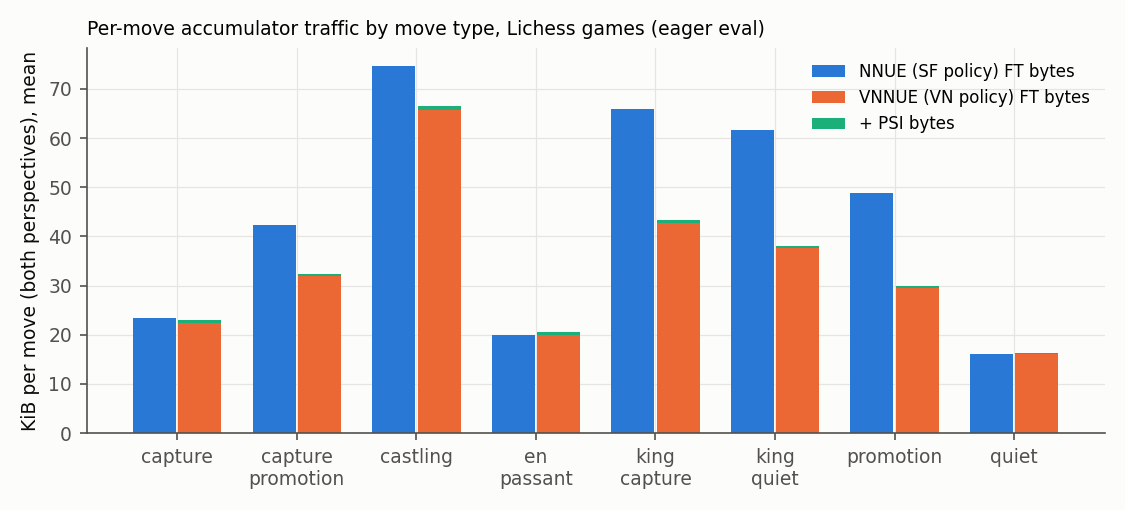
\includegraphics[width=0.85\linewidth]{figures/e2_bytes_per_move_type.png}
\caption{E2: per-move FT bytes, NNUE vs VNNUE, plus PSI bytes, by move type (Lichess games, eager; main run with a persisting Finny cache, so the king-move differences reflect our simulator, see Table~\ref{tab:reset}).}\label{fig:e2}
\end{figure}

\paragraph{Results.}
Tables~\ref{tab:movestats}--\ref{tab:e2} and Figure~\ref{fig:e2} show the results.
On a quiet move PSI adds exactly 4.69\% of PSQ column bytes, which is the T25 bound; the bound is tight at $k=2$.
Over all Lichess moves PSI adds 2.68\% of PSQ column bytes.
This drops to 1.75\% once NNUE's accumulator passes are counted (but not PSI's state pass, see above), and to 1.14\% once the threat proxy is counted (self-play: 2.62\%, 1.71\%, 1.19\%); the threat-proxy figures are computed on the first 600 Lichess games (36,701 moves).
On that subset the threat proxy changes 6.798 features per move and perspective on average, 2.98 times the number of changed piece-square features, slightly below the ``3--4$\times$ in a typical midgame'' stated in the nnue-pytorch documentation~\cite{nnuepytorchdocs}.
Own-king moves (quiet, captures and castling) are 13.1\% of Lichess moves (26,231 of 199,984).
In games, 8.94\% of accumulator builds need a table change (king bucket, mirror or block).
Hypothesis H1 (PSI overhead $\le4.7\%$ of PSQ column bytes) therefore holds under the byte model, which charges PSI for weight columns only.
Whether the extra bytes cost wall-clock time in an engine is not measured.

\subsection{E3: source selection and net-delta catch-up}\label{sec:e3}

We compare four policies, each simulated independently over the whole event stream with its own Finny caches and materialized accumulators:
\begin{itemize}[leftmargin=*,itemsep=1pt]
\item \textbf{SF}, a Stockfish-like rule: chain catch-up if there is no table change, otherwise hybrid if its conditions hold, otherwise Finny;
\item \textbf{SFmin}: chain catch-up whenever available (as SF), otherwise the argmin over \{refresh, Finny, hybrid\}; the SF-set minimum in Table~\ref{tab:e3cf} is defined the same way;
\item \textbf{VN\_noC4}, the argmin over \{refresh, Finny, hybrid, chain\}, i.e.\ SFmin except that it may skip an available chain;
\item \textbf{VN}, which is VN\_noC4 plus ancestor net-delta (C4).
\end{itemize}
The argmin scalar is $\mathrm{cols}+\mu\cdot\mathrm{mcols}+2\cdot\mathrm{passes}$.
Woodbury is not in these candidate sets; it is evaluated separately in E4.
\emph{Cache model.} In the main run (Tables~\ref{tab:e3}--\ref{tab:hybrid}) each policy keeps one Finny cache for the whole dataset, so entries persist across games and search trees and are updated only when a Finny, refresh or hybrid source is used.
They are therefore \emph{stale}, not cold: an entry may come from an unrelated game.
Stockfish clears its refresh table on \texttt{ucinewgame} and its cache is warmed by the search itself.
We therefore reran all four policies with the cache cleared at every root (each game and each search tree, warmed by the run itself; Table~\ref{tab:reset}).


\begin{table}[htbp]
\centering\small
\caption{E3 whole-trace totals per policy (stateful simulation).}\label{tab:e3}
\begin{tabular}{@{}llrrrrrr@{}}
\toprule
dataset & policy & \hd{cols/\\eval} & \hd{passes/\\eval} & \hd{FT bytes/\\eval} & \hd{cols\\vs SF} & \hd{passes\\vs SF} & \hd{PSI/FT\\bytes}\\
\midrule
games\_lichess/eager & SF & 7.841 & 2.079 & 24,576 & 1.0000 & 1.0000 & 1.75\%\\
 & SFmin & 6.438 & 2 & 21,377 & 0.8211 & 0.9618 & 2.02\%\\
 & VN\_noC4 & 6.436 & 2 & 21,373 & 0.8208 & 0.9618 & 2.02\%\\
 & VN & 6.436 & 2 & 21,373 & 0.8208 & 0.9618 & 2.02\%\\
\midrule
games\_selfplay/eager & SF & 7.877 & 2.102 & 24,744 & 1.0000 & 1.0000 & 1.71\%\\
 & SFmin & 6.382 & 2 & 21,263 & 0.8102 & 0.9513 & 1.99\%\\
 & VN\_noC4 & 6.38 & 2 & 21,257 & 0.8099 & 0.9513 & 1.99\%\\
 & VN & 6.379 & 2 & 21,256 & 0.8098 & 0.9513 & 1.99\%\\
\midrule
trees/eager & SF & 5.586 & 2.088 & 19,990 & 1.0000 & 1.0000 & 2.42\%\\
 & SFmin & 5.399 & 2 & 19,249 & 0.9666 & 0.9580 & 2.51\%\\
 & VN\_noC4 & 5.394 & 2 & 19,239 & 0.9656 & 0.9580 & 2.51\%\\
 & VN & 5.398 & 2 & 19,248 & 0.9665 & 0.9580 & 2.51\%\\
\midrule
trees/lazy & SF & 5.842 & 2.129 & 20,683 & 1.0000 & 1.0000 & 2.44\%\\
 & SFmin & 5.665 & 2.056 & 20,022 & 0.9697 & 0.9657 & 2.52\%\\
 & VN\_noC4 & 5.805 & 2.036 & 20,228 & 0.9938 & 0.9564 & 2.49\%\\
 & VN & 7.026 & 2 & 22,581 & 1.2027 & 0.9396 & 2.23\%\\
\bottomrule
\end{tabular}
\end{table}

\begin{table}[htbp]
\centering\small
\caption{Per-event counterfactual (T24 sanity check): at every build event, min over the full VN set $\le$ min over SF's set.}\label{tab:e3cf}
\begin{tabular}{@{}llcrr@{}}
\toprule
dataset & policy & \hd{holds at\\every event} & \hd{summed saving\\(col-equiv.)} & \hd{fraction of\\SF-set cost}\\
\midrule
games\_lichess/eager & VN\_noC4 & True & 347 & 0.02\%\\
games\_lichess/eager & VN & True & 534 & 0.03\%\\
games\_selfplay/eager & VN\_noC4 & True & 7 & 0.03\%\\
games\_selfplay/eager & VN & True & 9 & 0.04\%\\
trees/eager & VN\_noC4 & True & 3,335 & 0.09\%\\
trees/eager & VN & True & 3,760 & 0.10\%\\
trees/lazy & VN\_noC4 & True & 407,985 & 9.96\%\\
trees/lazy & VN & True & 948,711 & 18.73\%\\
\bottomrule
\end{tabular}
\end{table}

\begin{figure}[htbp]
\centering
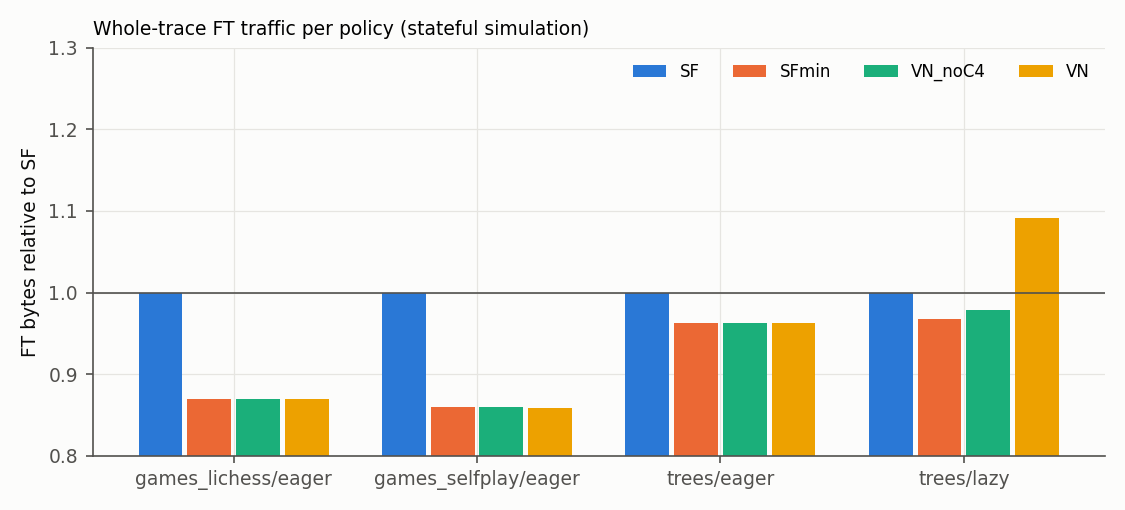
\includegraphics[width=0.8\linewidth]{figures/e3_policy_totals.png}
\caption{E3: whole-trace FT bytes per policy, relative to SF (main run, in which the Finny cache persists across games and trees; the SF/SFmin gap shrinks with a per-root reset, Table~\ref{tab:reset}).}\label{fig:e3}
\end{figure}

\paragraph{Results.}
Tables~\ref{tab:e3}--\ref{tab:e3cf} and Figure~\ref{fig:e3} show the results.
\begin{enumerate}[leftmargin=*,itemsep=2pt]
\item \emph{The never-worse property holds per event}, as T24 guarantees.
\item \emph{The superset adds almost nothing.}
In the eager runs, almost all of the gain of VN over the SF \emph{rule} comes from taking the argmin over SF's \emph{own} set (SFmin); on lazy trees VN is worse than SF (item~3).
SFmin and VN cost within 0.1\% of each other in the eager runs.
The per-event savings of VN over the SF-set minimum (at most 0.10\% in eager runs, Table~\ref{tab:e3cf}) come from VN being allowed to pick refresh, Finny or hybrid where SFmin is forced to chain, plus the ancestor candidate; Woodbury is not in these sets.
\item \emph{The size of the SFmin gain is a simulator artifact.}
In the main run the Finny cache persists across games and trees, so its entries are stale, and SF's hybrid rule is often more expensive than a plain Finny refresh: at table changes on Lichess games, hybrid averages 36.7 columns and Finny 16.3 (Table~\ref{tab:hybrid}).
With the cache cleared at every root (Table~\ref{tab:reset}), the column ratio of SFmin to SF on Lichess games rises from 0.8211 to 0.9387 (FT bytes 0.9466), and to 0.9780 on eager trees.
What remains comes from our model of the SF rule, which never chooses a plain refresh; with a reset cache, hybrid still averages 30.4 columns at table changes on Lichess games against 18.8 for Finny.
This is \textbf{not} evidence about Stockfish itself, whose hybrid conditions and cache warm-up we model only approximately, and it is no evidence that VNNUE saves bytes on king moves.
\item \emph{Greedy C4 hurts in a stateful search.}
On the lazy trees, VN uses 20.3\% more columns and 9.2\% more FT bytes per evaluation than SF, with 6\% fewer passes (with the cache reset per root: 1.2169 and 1.0992).
The cause is that C4 skips materializing intermediate accumulators that sibling nodes would later reuse.
The per-event counterfactual ``saving'' (18.73\%) is therefore misleading: the policies diverge in state, and per-event optimality does not compose.
Even without C4, VN\_noC4 is worse than SFmin on lazy trees (5.805 vs 5.665 cols/eval, 20,228 vs 20,022 FT bytes/eval) despite a 9.96\% per-event counterfactual saving, so the non-composition is a property of greedy argmin over the larger set, not only of C4.
\item \emph{Cancellation is larger than our prior.}
Within catch-ups of length $\ge2$ (227,886 events in the lazy run), cancellation saved 10.85\% of columns, with mean net-support ratio 0.905.
Stockfish's PR~\cite{sfpr5988} gives no figure for how much cancellation saves; its author estimated informally that about 0.2\% of three-move updates have one side moving the same piece twice, which is a different statistic from our column saving.
We attribute our higher saving to frequent same-square quiescence recaptures in our toy trees.
Our own prior H3 (column saving $<1\%$) is therefore not supported, but the whole-trace effect of greedy C4 is negative.
\end{enumerate}
A caveat: our ``lazy'' mode removed only 4\% of evaluations, because most nodes in these trees are quiescence nodes.

\begin{table}[htbp]
\centering\small
\caption{E3 rerun with the Finny cache cleared at every root (each game, each search tree), warmed by the run itself (\texttt{e3\_cache\_reset.py}; RESULTS.md \S2.7). Ratios are relative to SF in this rerun.}\label{tab:reset}
\begin{tabular}{@{}llrrrrr@{}}
\toprule
dataset & policy & \hd{cols/\\eval} & \hd{FT bytes/\\eval} & \hd{cols\\vs SF} & \hd{FT bytes\\vs SF} & \hd{per-event saving\\vs SF-set min}\\
\midrule
games\_lichess/eager & SF & 7.939 & 24,777 & 1.0000 & 1.0000 & \\
 & SFmin & 7.452 & 23,455 & 0.9387 & 0.9466 & \\
 & VN & 7.45 & 23,450 & 0.9384 & 0.9464 & 0.02\%\\
\midrule
games\_selfplay/eager & SF & 7.682 & 24,344 & 1.0000 & 1.0000 & \\
 & SFmin & 7.094 & 22,720 & 0.9234 & 0.9333 & \\
 & VN & 7.09 & 22,713 & 0.9230 & 0.9330 & 0.03\%\\
\midrule
trees/eager & SF & 5.527 & 19,870 & 1.0000 & 1.0000 & \\
 & SFmin & 5.405 & 19,262 & 0.9780 & 0.9694 & \\
 & VN & 5.406 & 19,263 & 0.9781 & 0.9695 & 0.11\%\\
\midrule
trees/lazy & SF & 5.78 & 20,555 & 1.0000 & 1.0000 & \\
 & SFmin & 5.671 & 20,034 & 0.9812 & 0.9746 & \\
 & VN\_noC4 & 5.811 & 20,240 & 1.0055 & 0.9847 & 9.96\%\\
 & VN & 7.033 & 22,595 & 1.2169 & 1.0992 & 18.72\%\\
\bottomrule
\end{tabular}
\par\smallskip
\begin{tabular}{@{}lrrrr@{}}
\toprule
Lichess games, per move & \hd{SF cols\\(main run)} & \hd{VN cols\\(main run)} & \hd{SF cols\\(reset)} & \hd{VN cols\\(reset)}\\
\midrule
king\_quiet & 25.332 & 14.822 & 19.48 & 14.874\\
king\_capture & 27.734 & 17.363 & 21.408 & 17.558\\
castling & 33.317 & 28.883 & 32.414 & 32.414\\
capture & 7.724 & 7.241 & 7.308 & 7.298\\
\bottomrule
\end{tabular}
\end{table}

\begin{table}[htbp]
\centering\small
\caption{Accumulator builds in the SF policy run (main run, Finny cache persisting across games and trees).}\label{tab:hybrid}
\begin{tabular}{@{}lrrrr@{}}
\toprule
dataset & builds & \hd{table-change\\builds} & \hd{SF Finny cols\\(mean/p50/p95)} & \hd{SF hybrid cols\\(mean/p50/p95)}\\
\midrule
games\_lichess/eager & 405,968 & 36,312 (8.94\%) & 16.289 / 16 / 35 & 36.683 / 36 / 65\\
games\_selfplay/eager & 4,880 & 519 (10.64\%) & 13.81 / 12 / 34.35 & 32.224 / 32 / 60.8\\
trees/eager & 779,328 & 52,504 (6.74\%) & 5.877 / 4 / 21 & 8.48 / 6 / 30\\
trees/lazy & 746,760 & 86,616 (11.60\%) & 4.635 / 4 / 10 & 8.436 / 7 / 28\\
\bottomrule
\end{tabular}
\end{table}

\subsection{E4: the low-rank king transition as a candidate}\label{sec:e4}

The Woodbury cost is $\mathrm{wb\_mult}\cdot r_K$ mcol $+|x_t\symd x_u|$ col $+1$ pass, where $\mathrm{wb\_mult}=2$ when $(U_{\kappa'}-U_\kappa)y$ is formed on the fly and $\mathrm{wb\_mult}=1$ when $\Delta U$ is precomputed.

\begin{table}[htbp]
\centering\small
\caption{E4 (Lichess games, eager; main run): fraction of own-king table-change events where Woodbury is the argmin. Totals relative to VN without Woodbury. ``col-equiv'' $=(\mathrm{cols}+\mu\cdot\mathrm{mcols})/\mathrm{cols}_{\mathrm{VN}}$; FT bytes count cols, mcols and passes. Tree rows are in RESULTS.md \S2.5.}\label{tab:e4}
\begin{tabular}{@{}rrrrrrrrr@{}}
\toprule
$r_K$ & $\mu$ & wb\_mult & \hd{Woodbury\\chosen} & \hd{total cols\\vs VN} & \hd{total\\mcols} & \hd{col-equiv\\vs VN} & \hd{FT bytes\\vs VN} & \hd{$y$-maint.\\lanes/make}\\
\midrule
4 & 1.0 & 2 & 59.7\% & 0.8052 & 125,208 & 0.9011 & 0.9390 & 22.706\\
4 & 1.5 & 2 & 44.4\% & 0.8357 & 93,224 & 0.9427 & 0.9427 & 22.706\\
4 & 2.0 & 2 & 30.7\% & 0.8734 & 64,528 & 0.9722 & 0.9524 & 22.706\\
8 & 1.0 & 2 & 30.7\% & 0.8734 & 129,056 & 0.9722 & 0.9828 & 45.411\\
8 & 1.5 & 2 & 6.9\% & 0.9667 & 28,768 & 0.9997 & 0.9930 & 45.411\\
8 & 2.0 & 2 & 0.0\% & 1.0000 & 0 & 1.0000 & 1.0000 & 45.411\\
16 & 1.0 & 1 & 30.7\% & 0.8734 & 129,056 & 0.9722 & 0.9828 & 90.823\\
16 & 1.0 & 2 & 0.0\% & 1.0000 & 0 & 1.0000 & 1.0000 & 90.823\\
16 & 1.5 & 1 & 6.9\% & 0.9667 & 28,768 & 0.9997 & 0.9930 & 90.823\\
16 & 1.5 & 2 & 0.0\% & 1.0000 & 0 & 1.0000 & 1.0000 & 90.823\\
16 & 2.0 & 1 & 0.0\% & 1.0000 & 0 & 1.0000 & 1.0000 & 90.823\\
16 & 2.0 & 2 & 0.0\% & 1.0000 & 0 & 1.0000 & 1.0000 & 90.823\\
\bottomrule
\end{tabular}
\end{table}

\begin{figure}[htbp]
\centering
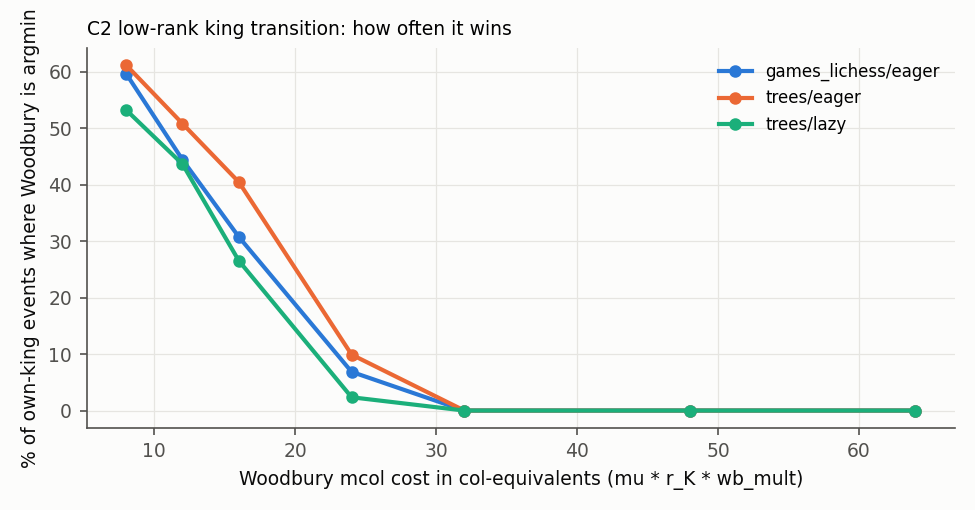
\includegraphics[width=0.75\linewidth]{figures/e4_woodbury_win_rate.png}
\caption{E4: Woodbury win rate at own-king events against its mcol cost $\mu\,r_K\,\mathrm{wb\_mult}$ in column equivalents.}\label{fig:e4}
\end{figure}

\paragraph{Results.}
Table~\ref{tab:e4} and Figure~\ref{fig:e4} show the results.
Woodbury is the argmin at own-king events only when $\mu r_K\,\mathrm{wb\_mult}\le24$ column-equivalents.
At the specification default ($r_K=16$, $\Delta U$ formed on the fly) it won 0\% of own-king events for every $\mu\in\{1,1.5,2\}$ on every swept dataset (Lichess games, eager and lazy trees; self-play was not swept).
This is consistent with hypothesis H2.
With precomputed $\Delta U$ at $\mu=1$ it wins 30.7\% of own-king events on Lichess games and uses 12.7\% fewer plain columns, but it adds 129,056 mcols, so the col-equivalent ratio is 0.9722 and FT bytes fall only 1.7\% (ratio 0.9828; 21,005.8 vs 21,372.8\,B per evaluation).
That also requires about 91 extra $y$-maintenance lanes per make event and a precomputed $\Delta U$ table (about 18.5\,MB, Section~\ref{sec:arch}).
On search trees Woodbury lowers column count slightly (0.9749 at $r_K=4$, $\mu=1$, eager) but increases FT bytes (ratio 1.0250 eager, 1.0596 lazy) once its mcols are counted (RESULTS.md \S2.5).
The cache-reset rerun gives the same picture: 0.9784 of VN's FT bytes on Lichess games at $r_K=16$ with precomputed $\Delta U$, and 1.0420 on eager trees (RESULTS.md \S2.7).

\subsection{E5: cost of the low-rank integer factorization}\label{sec:e5}

We used a synthetic planted table: one block, 32 buckets, 704 features and 256 lanes, with $W_k=W^0+U_kV$ (true rank 8) plus Gaussian noise, and an unstructured control.
$V_K$ is the top-$r_K$ right singular subspace of the stacked residuals.
In ``int factors'', $V_K$ is quantized to int8 and $U$ to int16 so that $UV_K$ is in table units at scale 64, and the integer product is materialized (the C2 exactness requirement).

\begin{table}[htbp]
\centering\small
\caption{E5: relative squared Frobenius error of the per-bucket residual (selected $r_K$; full table in \texttt{RESULTS.md}).}\label{tab:e5}
\begin{tabular}{@{}lrrrr@{}}
\toprule
table & $r_K$ & float SVD & \hd{int factors\\(materialized)} & \hd{plain int16\\table}\\
\midrule
planted\_rank8\_noise0.1 & 4 & 0.466 & 0.57 & 2.08e-05\\
 & 8 & 0.00978 & 0.218 & 2.08e-05\\
 & 16 & 0.0096 & 0.18 & 2.08e-05\\
 & 64 & 0.00856 & 0.164 & 2.08e-05\\
planted\_rank8\_noise0.5 & 8 & 0.195 & 0.315 & 1.65e-05\\
 & 16 & 0.191 & 0.315 & 1.65e-05\\
unstructured & 8 & 0.981 & 1 & 2.1e-05\\
 & 16 & 0.963 & 1 & 2.1e-05\\
 & 64 & 0.86 & 1 & 2.1e-05\\
\bottomrule
\end{tabular}
\end{table}

\begin{figure}[htbp]
\centering
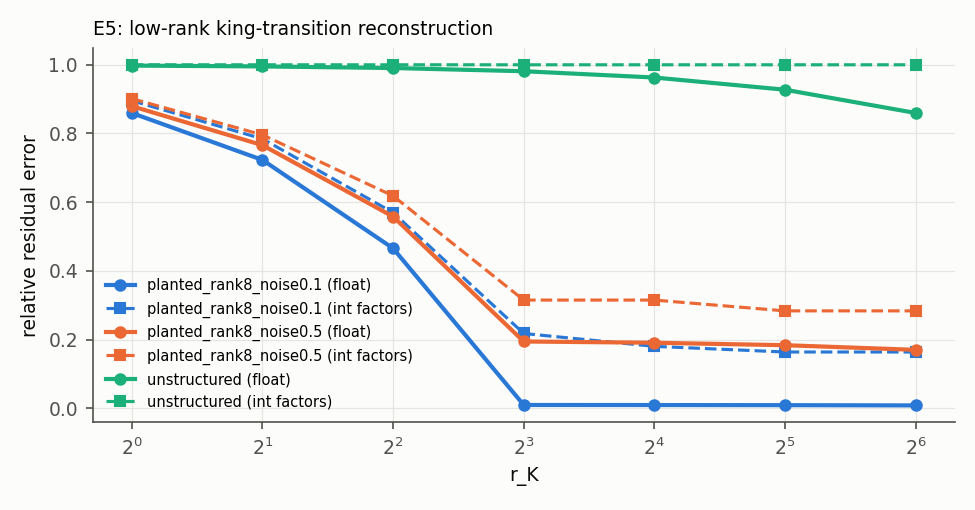
\includegraphics[width=0.8\linewidth]{figures/e5_rank.png}
\caption{E5: low-rank reconstruction error against $r_K$, float vs integer factors.}\label{fig:e5}
\end{figure}

\paragraph{Results.}
Table~\ref{tab:e5} and Figure~\ref{fig:e5} show the results.
On the planted rank-8 table, rank 8 recovers the residual in float (relative error 0.00978).
Rounding $U$ and $V_K$ so that their product is exact raises the error to 0.218, against 2.08e-05 for a plain int16 table at the same scale.
Without QAT, the integer-factor constraint is expensive.
On an unstructured table low rank does not help at all.
This experiment complements \texttt{lowrank\_proper} (T23).

\subsection{E6--E8: small training sanity checks}\label{sec:training}

\paragraph{Configuration.}
All models were trained for 6 epochs with batch size 1024 and Adam with a one-cycle schedule (max\_lr 2e-3), on seeds 0, 1, 2.
They use a single White-absolute perspective, no king buckets and no layer stacks.
The 175,984 Lichess positions (ply $\ge8$) were split by game into 140,307 training and 35,677 validation positions.
The synthetic teachers are $y=z(\mathrm{PST}\cdot\beta)+z(\text{pair term})+\text{noise}$, standardized to unit variance.
The pair term is (i) a low-rank $Q$ (rank 8, dense), (ii) a sparse ``attack-geometry'' $Q$ with 72,590 nonzero pairs, or (iii) both.
The models are listed below.
\begin{itemize}[leftmargin=*,itemsep=1pt]
\item M0\_L256 (201,281 parameters, 256 update lanes per changed feature).
\item M0s\_L192 (150,977 parameters, 192 lanes).
\item M1\_L192\_PSI\_r32\_m16 (176,593 parameters, 256 lanes). This model is matched to M0\_L256 in update lanes, not in bytes ($P2$ lanes are int32: $192\cdot2+32\cdot2+32\cdot4=576$\,B against 512\,B per changed feature) and not in readout MACs, which M0 does not pay.
\item M2\_L192\_explicit\_pairs (14,088,449 parameters). It also updates $L$ lanes for each changed active pair, of which there are on average 40.044 per position. M2 is a non-cost-matched reference with oracle knowledge of teacher (ii)'s support, run with 1 seed.
\end{itemize}

\begin{table}[htbp]
\centering\small
\caption{E6: held-out MSE (mean $\pm$ sample s.d.\ over 3 seeds; M2 one seed).}\label{tab:e6}
\begin{tabular}{@{}lrrrr@{}}
\toprule
teacher & M0\_L256 & M0s\_L192 & M1 (PSI) & M2 (explicit pairs)\\
\midrule
i\_lowrank & 0.0666 $\pm$ 0.0025 & 0.0706 $\pm$ 0.0022 & \textbf{0.0389} $\pm$ 0.0031 & 0.1476\\
ii\_sparse\_attack & 0.1607 $\pm$ 0.0003 & 0.1691 $\pm$ 0.0015 & 0.1487 $\pm$ 0.0035 & \textbf{0.0424}\\
iii\_both & 0.1612 $\pm$ 0.0022 & 0.1672 $\pm$ 0.0049 & 0.1336 $\pm$ 0.0020 & \textbf{0.1222}\\
\bottomrule
\end{tabular}
\end{table}

\begin{figure}[htbp]
\centering
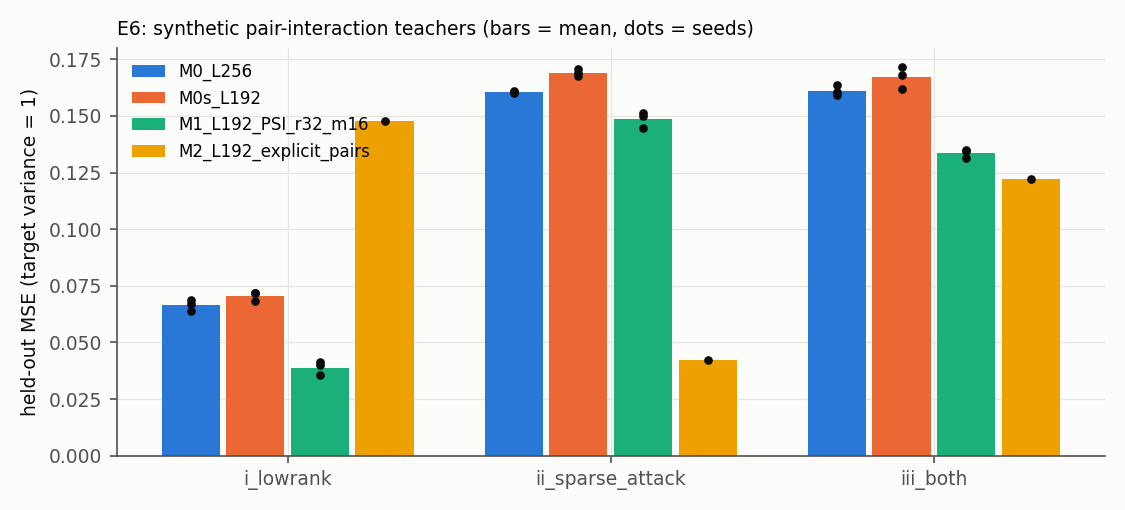
\includegraphics[width=0.8\linewidth]{figures/e6_training.png}
\caption{E6: held-out MSE per synthetic teacher and model.}\label{fig:e6}
\end{figure}

\paragraph{E6 results.}
Table~\ref{tab:e6} and Figure~\ref{fig:e6} show the results.
On all three synthetic pair teachers, the cost-matched M1 had lower held-out MSE than M0 and M0s.
The explicit-pair reference M2 is best on the sparse-attack teacher and on ``both'', and worst on the low-rank teacher; that last result is a single seed with a 14-million-parameter table and is likely undertrained, so it is not a meaningful comparison.
These teachers were \emph{built} to contain pair structure.
The result shows that PSI can learn such structure and nothing about chess evaluation.

\paragraph{Quantized PSI readout.}
We took M1 trained on teacher (iii), seed 0, quantized $V$ and $\Lambda$ to int8, and evaluated it on 4,000 validation positions.
The maximum $|P1|$ was 571 (bound 4064) and the maximum $P2$ was 43,527 (bound 516,128).
$P1^2-P2$ was even everywhere, and the maximum $|z_{\mathrm{int}}|$ was 21,117,603, below $2^{31}$.
The integer pipeline equalled a float evaluation of the quantized weights, and quantization gave a relative RMS error of 0.0161 in $z$.

\begin{table}[htbp]
\centering\small
\caption{E7 (tying under colour flip) and E8 (real-ish labels): held-out MSE.}\label{tab:e78}
\begin{tabular}{@{}llrr@{}}
\toprule
\multicolumn{4}{@{}l}{\emph{E7: M1, tied vs untied $V$} (untied 176,593 params, tied 164,305)}\\
teacher & & untied & tied\\
\midrule
iii\_both & & 0.1337 $\pm$ 0.0020 & 0.1498 $\pm$ 0.0062\\
iii\_both\_colour\_symmetrised & & 0.1362 $\pm$ 0.0029 & 0.1209 $\pm$ 0.0013\\
\midrule
\multicolumn{4}{@{}l}{\emph{E8: real-ish labels}}\\
label & mean predictor & M0\_L256 / M0s\_L192 & M1 (PSI)\\
\midrule
game\_result\_white\_pov & 0.2412 & 0.2807 $\pm$ 0.0030 / 0.2809 $\pm$ 0.0037 & 0.2920 $\pm$ 0.0022\\
material\_pst\_eval\_tanh & 0.3025 & 0.0158 $\pm$ 0.0008 / 0.0155 $\pm$ 0.0015 & 0.0158 $\pm$ 0.0023\\
\bottomrule
\end{tabular}
\end{table}

\paragraph{E7 and E8 results.}
Table~\ref{tab:e78} shows the results.
E7 retrains the untied M1 separately; the 0.0001 difference from Table~\ref{tab:e6} (0.1337 vs 0.1336) is run-to-run nondeterminism.
Tying $V$ under the colour flip \emph{hurt} on a teacher that is not colour-symmetric and helped on a colour-symmetrized one.
T21 held exactly on the trained tied model: the maximum $|P1(\text{flipped})-P1[\text{perm}]|$ and $|P2(\text{flipped})-P2[\text{perm}]|$ were both $0.00$.
On game results, every model was \emph{worse} than predicting the training mean, so this data and label combination is too small and noisy to compare models on. PSI was the worst.
On a linear material+PST label all models tie, as expected, because PSI has nothing to add to a label that is linear in $\beta$.
\textbf{No real-label benefit of PSI was observed.}

\subsection{Wall-clock proxy}

Table~\ref{tab:bench} gives the timings.
They were taken with Python on a 138.4\,MB int16 table (single thread, median of 5).
Unbatched timings measure Python dispatch more than memory traffic.
In batched torch kernels, a PSI quiet-move update costs 0.066 of an NNUE quiet-move update (4 columns), against a byte ratio of $384/8192=0.047$.
None of these timings predicts engine nps.

\begin{table}[htbp]
\centering\small
\caption{Wall-clock microbenchmark (rough proxy only; not engine speed).}\label{tab:bench}
\begin{tabular}{@{}lr@{\qquad}lrr@{}}
\toprule
unbatched kernel & ns/event & batched kernel & ns/event & GB/s\\
\midrule
NNUE quiet move, both persp., 4 cols & 9,572 & NNUE quiet, 4 cols & 7,578 & 1.081\\
PSI quiet move $P1,P2$ & 5,360 & PSI quiet $P1,P2$ & 503.502 & 0.763\\
refresh, 32 cols, one persp. & 49,841 & refresh, 32 cols & 46,933 & 1.396\\
Woodbury $r_K=16$ + 2 cols, one persp. & 39,960 & & &\\
PSI readout, one persp., $m=16$ & 27,140 & & &\\
\bottomrule
\end{tabular}
\end{table}

\subsection{Limitations of the experiments}
\begin{itemize}[leftmargin=*,itemsep=1pt]
\item The K32H3 model is simplified: threat and pawn-pair columns are not in the accumulator (threat bytes come from a proxy and are only counted), and there are no PSQT outputs and no layer stacks.
\item Search traces come from a toy alpha-beta (depth 3 + quiescence, 2,500-node cap, 116 of 200 trees truncated), not from Stockfish. Catch-up lengths, king-move frequencies and cache warmth are proxies.
\item The Stockfish policy is modelled from the specification text. The backward catch-up fill after a Finny refresh is not modelled, and pass costs are a uniform $4L$ bytes.
\item In the main E2--E4 run the Finny cache persists across games and trees (Section~\ref{sec:e3}); the rerun with a per-root reset changes the SF/SFmin ratios substantially but not the qualitative conclusions.
\item E1 covers subsets of the data (Section~\ref{sec:e1}).

\item Training uses one perspective, no king buckets, 6 epochs on 140k positions and synthetic teachers. M2 used 1 seed. E5 uses post-training quantization of the factors, not QAT.
\item Wall clock comes from Python on a 4\,GB laptop.
\end{itemize}

%=====================================================================
\section{Discussion}\label{sec:discussion}
%=====================================================================

\paragraph{What worked.}
\begin{itemize}[leftmargin=*,itemsep=2pt]
\item \emph{The algebraic view is right and checkable.}
For a fixed weight table, the \emph{correctness} of every accumulator mechanism we examined is an instance of a few identities in a homomorphism $\Z^N\to R^L$: T1--T3, T23, T24(b).
This holds for incremental updates, Finny caches, the hybrid update, lazy catch-up and low-rank transitions.
Instantiating at $R=\Zm{16}$ makes wrap-around exactness a corollary rather than a folklore observation, and E1 confirmed bit-exactness on 14.5 million checks (6.67M accumulator-source, 7.80M PSI/$y$/feature-delta), including 58 million lane results whose paths overflowed.
\item \emph{PSI is cheap and exact as an update.}
Its per-move weight-column traffic is bounded by a proved 4.6875\% of PSQ column traffic and measured at 2.68\% over real games (1.14\% with the threat proxy, on the first 600 games); these ratios exclude PSI's own state pass.
It never needs a refresh.
Its integer readout is exact over $\Z$ (T12), and the exact $P1$, $P2$ and head sums are within int16/int32 (T9, T16).
Wrapping $\Zm{32}$ semantics for $P2$ and the bias $b^z$ are not covered by Lean.
\item \emph{Formalization caught errors in our own specification.}
The \texttt{valMinAbs} window, saturation path dependence, the missing hypotheses in the degree-3 range, the false ``$V=I$'' universality claim, the false affinity claim, and the low-rank expressiveness reading were all caught and corrected before implementation.
These were errors in our design document; several are known facts (Mathlib's documented \texttt{valMinAbs} convention, the reason Stockfish uses wrapping adds, an elementary rank argument), not findings about NNUE.
\end{itemize}

\paragraph{What did not work, or not yet.}
\begin{itemize}[leftmargin=*,itemsep=2pt]
\item \emph{``Never worse'' is true but nearly vacuous in practice.}
T24 is min-monotonicity.
Empirically the extra freedom in the VN set (choosing refresh, Finny or hybrid instead of a forced chain, plus the ancestor candidate) contributed at most 0.10\% per-event savings in eager runs (Table~\ref{tab:e3cf}); Woodbury was not in the E3 sets and was evaluated separately (E4, Section~\ref{sec:e4}).
The visible gain of VN over the SF rule comes from taking the argmin over SF's own set, which would equally improve Stockfish, and its size depends on our simulator's cache model (Section~\ref{sec:e3}).
\item \emph{Greedy net-delta catch-up is harmful.}
Per-event optimality does not compose across a stateful search, and skipping materialization destroys reuse by siblings.
On lazy trees even VN\_noC4, without C4, is worse than SFmin.
C4 would need a reuse-aware policy, for example one guided by the ski-rental analysis (A1), before it could help.
\item \emph{Low-rank king transitions rarely win.}
At the specification default they never won.
They win own-king events only with a precomputed $\Delta U$ table (about 18.5\,MB) or very small $r_K$, and even then the net saving is small once their multiply-add columns are counted: on Lichess games at $r_K=16$ with precomputed $\Delta U$, FT bytes fall only to 0.9828 of VN's, and on search trees they rise.
E5 shows that the exact integer-factor constraint costs a lot of accuracy without QAT.
\item \emph{PSI has no demonstrated benefit on chess labels.}
It learned planted pair structure (E6), but on game results all models were worse than the mean predictor, and on a linear label PSI has nothing to add.
Our data is too small to say anything about real evaluation quality.
\item \emph{Tying is a prior, not a free lunch.}
Colour-flip tying of $V$ halves the free parameters of $V$ (the state is shared by both perspectives with or without tying), but it hurt on a non-symmetric teacher (E7).
\end{itemize}

\paragraph{What would establish an improvement.}
Whether VNNUE improves an engine depends on two quantities we cannot measure here.
The first is the change in evaluation accuracy at fixed compute, for networks trained on Stockfish-scale data (billions of positions with Leela-rescored labels).
The second is the change in node rate caused by the added PSI bytes and readout MACs on real SIMD hardware.
Establishing an improvement would require the following steps:
\begin{enumerate}[leftmargin=*,itemsep=1pt]
\item a C++ implementation of C1 (and optionally C3) in Stockfish, with perf-counter measurements of nps, cache misses and bytes per node on AVX2, AVX-512 and NEON;
\item training K32H3+PSI with the full nnue-pytorch pipeline and quantization-aware training, against an identically trained K32H3 baseline, and comparing validation loss at equal measured nps;
\item an ablation over $r\in\{0,8,16,32\}$, $m\in\{0,8,16\}$, degree, tying, and the C2/C6 modes;
\item fixed-node matches, followed by fixed-time SPRT~\cite{wald1945} at two time controls on Fishtest-like infrastructure~\cite{fishtest}.
\end{enumerate}
Until then, VNNUE should be read as a verified design whose costs are bounded and whose benefits are hypotheses.

\paragraph{Threats to validity of the formal results.}
The Lean development proves statements about abstract index sets and lane groups.
Its connection to engine code rests on informal modelling: the feature map, the move-delta table, and the cost model.
E1 tests the Python prototype, not Stockfish.
The cost theorems (T24, T25) are only as meaningful as their cost functions.

%=====================================================================
\section{Related work}\label{sec:related}
%=====================================================================

\paragraph{NNUE.}
NNUE was introduced by Nasu~\cite{nasu2018} and documented for chess in the nnue-pytorch documentation~\cite{nnuepytorchdocs}.
Its engineering in Stockfish includes Finny tables~\cite{sffinny}, two-ply cancellation~\cite{sfpr5988}, threat inputs~\cite{sfthreats,sfsource}, larger and then smaller L1~\cite{pr5149}, the dual-net period~\cite{pr4915}, K32Q2~\cite{sfnnv18} and K32H3~\cite{pr563}.
This is the direct baseline, and all of the mechanisms we formalize in T1--T11 and T24(b) are credited prior art.
Our contribution there is the exact statement and machine-checked proof, not the mechanism.
The bullet trainer~\cite{bullet} and other engines use similar input-bucket designs; the Stockfish threat-input change itself credits prior threat-input work in Monty, PlentyChess and Yukari~\cite{sfthreats}.
nnue-pytorch's feature factorization (shared virtual features merged into king-bucketed weights at export)~\cite{nnuepytorchdocs} is the full-rank, training-time precursor of C2.
We have not surveyed every engine, and pairwise interaction ideas may exist in community engines that we are not aware of.

\paragraph{Incremental computation.}
Finite differencing~\cite{paige1982}, self-adjusting computation~\cite{acar2002}, change theories~\cite{cai2014} and DBSP~\cite{budiu2023} provide general frameworks.
NNUE is a particularly clean instance: the derivative of a linear map is the map itself.
Delta networks~\cite{neil2017} and DeltaCNN~\cite{parger2022} apply temporal sparsity to deep networks.
They accept approximation, whereas we insist on bit-exactness.

\paragraph{Interactions and set functions.}
Factorization machines~\cite{rendle2010} and their higher-order variants~\cite{blondel2016} compute pairwise (and higher) interactions from power sums. Tensor decompositions~\cite{kolda2009} are the general low-rank language.
Deep Sets~\cite{zaheer2017} show that sum-of-embeddings pooling is the canonical permutation-invariant architecture (on countable domains).
In chess, pairwise piece terms predate NNUE: material-imbalance polynomials~\cite{kaufman1999,sf11}, and in NNUE the FT pairwise product and the threat and pawn-pair features.
PSI's contribution is a parametrization: a refresh-free power-sum state for square-level pair interactions that complements the FT's clipped rank-one products, with pre-shift head values that form a factorization machine.

\paragraph{Symmetry.}
Group-equivariant networks~\cite{cohen2016} and equivariance through parameter sharing~\cite{ravanbakhsh2017} give the framework of T21--T22.
Stockfish's perspective flip and horizontal mirroring are special cases.

\paragraph{Low rank.}
nnue-pytorch's factorizer~\cite{nnuepytorchdocs} ($W_\kappa=R_\kappa+Q$, merged at export) is the direct precursor of C2; C2 restricts the bucket-specific part to rank $r_K$ so that it can be applied incrementally at inference, and \lnm{lowrank_generalizes} is the full-rank case.
The low-rank-correction pattern is also that of Sherman--Morrison--Woodbury~\cite{sherman1950,woodbury1950} (which concerns inverses) and LoRA~\cite{hu2022lora}.
Our negative result \texttt{lowrank\_proper} is the elementary rank argument that limits all such schemes.

\paragraph{Quantization and formal methods.}
Integer-only inference~\cite{jacob2018} and rounding analysis~\cite{higham2002} underlie C5.
We are not aware of prior machine-checked proofs about NNUE accumulators.
The formalization uses Lean~4~\cite{demoura2021} and Mathlib~\cite{mathlib2020}.

%=====================================================================
\section{Conclusion and future work}\label{sec:conclusion}
%=====================================================================

We recast NNUE accumulator maintenance as an exact update calculus over the delta group $\Z^N\to(\Zm{16})^L$ and formalized it in Lean~4: 149 theorem declarations and a full build with no \texttt{sorry}; the axiom audit of all 149 declarations shows only \texttt{propext}, \texttt{Classical.choice} and \texttt{Quot.sound}.
On top of it we designed VNNUE.
VNNUE keeps Stockfish's FT, adds a refresh-free power-sum interaction channel whose pre-shift head values form an all-pairs factorization machine, and replaces rule-based accumulator sourcing with a min-cost selection over a superset of Stockfish's candidates.
The update mechanics are exact (14.5 million checks: 6.67M accumulator-source and 7.80M PSI/$y$/feature-delta, 0 mismatches) and cheap in weight-column traffic (PSI adds 2.68\% of PSQ column bytes on real games, not counting its own state pass).

The proposed efficiency gains beyond Stockfish's existing machinery are essentially absent (C3 superset), harmful (greedy C4) or conditional on unattractive trade-offs (C2).
The accuracy benefit of PSI on chess is unknown.

The next steps follow directly from this.
The first is to implement C1 in Stockfish's C++ with SIMD, and to measure nps and bytes per node.
The second is to train K32H3+PSI at scale with QAT and compare validation loss at equal nps.
The third is to test with SPRT on Fishtest.
On the theory side, the obvious extensions are to formalize a reuse-aware materialization policy for catch-up, to connect the abstract index sets to a verified K32H3 feature map, and to state explicit $\Zm{32}$ instances and an int32 decode lemma for the PSI state. The generic theorems already hold over any abelian group, but the development instantiates them only at $\Z$ and $\Zm{16}$.

\paragraph{Code and data availability.}
All Lean sources, the Modal-based proof checker, the experiment scripts, derived datasets, raw result files, figures and the \LaTeX{} sources of this paper are available at \url{https://github.com/HelloTest006/vnnue}.
The raw Lichess game file is not redistributed; it is available under CC0 from \url{https://database.lichess.org}.

\paragraph{Acknowledgments and use of AI tools.}
The research notes, design, Lean formalization, experiment code and drafts of this paper were produced with substantial assistance from an AI system (Claude, by Anthropic), operating under the author's direction.
Every theorem cited as proved is checked by the Lean kernel (Appendix~\ref{app:lean}), and every reported number is produced by the published scripts.
The author takes full responsibility for the content.

\bibliographystyle{plainnat}
\bibliography{refs}

\appendix

%=====================================================================
\section{Lean development overview}\label{app:lean}
%=====================================================================

\paragraph{Toolchain.}
The development uses Lean \texttt{leanprover/lean4:v4.35.0} and Mathlib tag \texttt{v4.35.0}, with a Lake project \texttt{vnnue} and library \texttt{VNNUE}.
The root file \texttt{VNNUE.lean} imports the eight modules.
\texttt{Basic} imports only Mathlib, and every other module imports only Mathlib and \texttt{VNNUE.Basic}.
For this reason a few facts are re-proved locally under distinct names: \lnm{quant_foldDeltas_eq} in \texttt{Quantization}, \lnm{refresh_accS_any_source} in \texttt{Refresh}, and \lnm{inf'_superset_cx} in \texttt{Complexity}.

\begin{table}[h]
\centering\small
\caption{Modules. ``Decls'' counts \texttt{theorem}/\texttt{lemma} declarations in the source; ``audited'' counts those whose \texttt{\#print axioms} output appears in the build log.}\label{tab:modules}
\begin{tabular}{@{}llrrr@{}}
\toprule
Module & Spec IDs & Lines & Decls & Audited\\
\midrule
\texttt{Basic} & definitions + sanity lemmas & 131 & 11 & 11\\
\texttt{Accumulator} & T1--T3 & 187 & 18 & 18\\
\texttt{DeltaMonoid} & T4--T6 & 96 & 8 & 8\\
\texttt{Quantization} & T7--T11 & 289 & 25 & 25\\
\texttt{Interaction} & T12--T18 & 432 & 27 & 27\\
\texttt{Symmetry} & T19--T22 & 359 & 31 & 31\\
\texttt{Refresh} & T23--T24 & 254 & 18 & 18\\
\texttt{Complexity} & T25, A1, A2 & 151 & 11 & 11\\
\texttt{VNNUE.lean} (root) & imports & 8 & 0 & 0\\
\midrule
Total & & 1,907 & 149 & 149\\
\bottomrule
\end{tabular}
\end{table}

\paragraph{Axiom audit.}
The checker \texttt{lean/modal\_check.py} runs \texttt{lake build} on a Modal CPU container with the Mathlib cache.
It then writes an audit file containing \texttt{\#print axioms} for every \texttt{theorem}/\texttt{lemma} declaration (including those preceded by an attribute such as \texttt{@[simp]}), and compiles that file.
The resulting log (\texttt{full\_check.log}) ends with \texttt{RESULT: OK}.
It contains 149 audit lines, one per theorem declaration, with the following breakdown:
\begin{itemize}[leftmargin=*,itemsep=1pt]
\item 127 declarations depend on \{\texttt{propext}, \texttt{Classical.choice}, \texttt{Quot.sound}\};
\item 19 on \{\texttt{propext}, \texttt{Quot.sound}\};
\item 2 on \{\texttt{propext}\};
\item 1 (\lnm{sat16_eq_clampZ}, proved by \texttt{rfl}) on no axioms.
\end{itemize}
So all 149 theorem declarations use at most the three standard axioms, and none uses \texttt{sorryAx}.
The build log shows only linter warnings: the \texttt{module}-system hint for files that import Mathlib, deprecations of \texttt{push\_neg}, \texttt{if\_pos} and \texttt{if\_neg}, eight unused-simp-argument warnings (in \texttt{Interaction}), and one unused variable.
No \texttt{native\_decide} is used anywhere.

\paragraph{Documented deviations from the specification.}
(1)~\texttt{deriving Fintype} for \texttt{Src} fails on this toolchain. It is replaced by a hand-written instance with a \texttt{decide} check that the type has 6 elements.
(2)~T17 uses $N^2$ pair lanes rather than $\binom N2$.
(3)~T23 adds \lnm{lowrank_proper} (square $L=n$ tables over a field) and its rational instance, which refute the expressiveness-preservation reading of \lnm{lowrank_generalizes}; the extension to the deployed $1024\times704$ integer tables is informal.

(4)~T24 adds \lnm{never_worse_dominated} (two cost functions) and \lnm{hybrid_correct_impl} (Stockfish's evaluation order), so that the assumptions of the specification's single-cost form are explicit.
(5)~T19 adds \lnm{king_half_onto}, and T20 adds \lnm{canon_mem_orbit} and \lnm{canon_eq_iff}, so that ``192 orbits'' is actually derived rather than just ``192 canonical values''.
(6)~T21 adds \lnm{acc_equivariant_accV} (with bias) and \lnm{psi_shared_sigC} (the concrete colour flip, all powers $k$).
(7)~T22 adds \lnm{isotypic_action}, \lnm{isotypic_inj} and \lnm{isotypic_not_surj}.

\paragraph{Reproducing.}
\begin{verbatim}
cd lean
modal run modal_check.py                    # all modules + root, prints RESULT
modal run modal_check.py --files VNNUE/Basic.lean,VNNUE/Accumulator.lean
\end{verbatim}
The image clones Mathlib \texttt{v4.35.0}, installs \texttt{elan}, and fetches the prebuilt cache (\texttt{lake exe cache get}).
On a machine with roughly 8\,GB of free RAM the development can also be checked locally with \texttt{cd lean \&\& lake exe cache get \&\& lake build}; the Mathlib revision is pinned in \texttt{lakefile.toml} and \texttt{lake-manifest.json}.
A full run builds the 8 modules in about 20--45\,s each on 8 vCPUs.

%=====================================================================
\section{Full theorem index}\label{app:index}
%=====================================================================

All names are in namespace \texttt{VNNUE}.
``(h)'' marks helper lemmas that support a spec theorem; ``(i)'' marks instantiations at $\Z$ or $\Zm{16}$ (\texttt{ZMod 65536}).
Statements are abbreviated, and Section~\ref{sec:theorems} gives them in full.

{\small
\begin{longtable}{@{}p{1.1cm}p{5.3cm}p{8.6cm}@{}}
\toprule
ID & Lean name & Statement\\
\midrule
\endfirsthead
\toprule
ID & Lean name & Statement\\
\midrule
\endhead
\bottomrule
\endfoot
\multicolumn{3}{@{}l}{\emph{Basic (sanity lemmas)}}\\
-- & \lean{ind_apply} & $\one_S(i)=[i\in S]$\\
-- & \lean{ind_of_mem}, \lean{ind_of_not_mem} & $\one_S(i)=1$ if $i\in S$; $=0$ if $i\notin S$\\
-- & \lean{ind_isBinary} & $\one_S$ is binary\\
-- & \lean{delta_apply} & $\delta(S,T)_i=\one_T(i)-\one_S(i)$\\
-- & \lean{mem_supp} & $i\in\supp\delta\iff\delta_i\ne0$\\
-- & \lean{foldDeltas_nil}, \lean{foldDeltas_cons} & fold of $[]$ is identity; one fold step\\
-- & \lean{dec16_intCast_of_inI16} & $\dec(v)=v$ on int16 range\\
-- & \lean{sat16_of_inI16} & $\satop v=v$ on int16 range\\
-- & \lean{sat16_eq_clampZ} & $\satop=\clamp(-32768,32767,\cdot)$\\
\midrule
\multicolumn{3}{@{}l}{\emph{Accumulator}}\\
T1 & \lean{Phi_add} & $\Phi_W(x+y)=\Phi_Wx+\Phi_Wy$\\
T1 & \lean{accV_add_delta} & $\accV(x+\delta)=\accV(x)+\Phi_W\delta$\\
T1 & \lean{Phi_eq_sum_supp} & $\Phi_W\delta=\sum_{i\in\supp\delta}\delta_iW_i$\\
T2 & \lean{foldDeltas_eq} & $\fold(\accV x,\ell)=\accV(x+\sum\ell)$\\
T2 & \lean{foldDeltas_perm} & fold is invariant under permutation of $\ell$\\
T2 (h) & \lean{foldDeltas_append} & fold over $\ell_1\mathbin{+\!\!+}\ell_2$ = fold $\ell_2$ after fold $\ell_1$\\
T2 (h) & \lean{foldDeltas_group} & a prefix may be replaced by its net delta\\
T3 & \lean{accS_eq_accV} & $\accS(S)=\accV(\one_S)$\\
T3 & \lean{accS_any_source} & $\accS(S)=\accS(U)+\sum_{S\setminus U}W-\sum_{U\setminus S}W$\\
T3 & \lean{colOps_eq} & $|S\symd U|=|S\setminus U|+|U\setminus S|$\\
T3 (h) & \lean{Phi_delta} & $\Phi_W\delta(U,S)=\sum_{S\setminus U}W-\sum_{U\setminus S}W$\\
T1 (i) & \lean{accV_add_delta_int}, \lean{accV_add_delta_zmod} & T1(b) at $\Z$, $\Zm{16}$\\
T2 (i) & \lean{foldDeltas_eq_int}, \lean{foldDeltas_eq_zmod} & T2(a) at $\Z$, $\Zm{16}$\\
T3 (i) & \lean{accS_any_source_int}, \lean{accS_any_source_zmod} & T3(b) at $\Z$, $\Zm{16}$\\
T3/T7 (h) & \lean{castLanes_accV_int} & lane-wise cast commutes with $\accV$\\
\midrule
\multicolumn{3}{@{}l}{\emph{DeltaMonoid}}\\
T4 & \lean{delta_telescope} & $\delta(S_0,S_1)+\delta(S_1,S_2)=\delta(S_0,S_2)$\\
T4 & \lean{ind_add_delta} & $\one_S+\delta(S,T)=\one_T$\\
T4 & \lean{supp_delta} & $\supp\delta(S,T)=S\symd T$\\
T5 & \lean{supp_add_subset} & $\supp(\delta+\varepsilon)\subseteq\supp\delta\cup\supp\varepsilon$\\
T5 & \lean{card_supp_sum_le} & $|\supp\sum\ell|\le\sum|\supp\delta_j|$\\
T6 & \lean{colOps_triangle} & triangle inequality for $|\cdot\symd\cdot|$\\
T6 & \lean{colOps_comm} & symmetry\\
T6 & \lean{colOps_image} & invariance under injective relabelling\\
\midrule
\multicolumn{3}{@{}l}{\emph{Quantization}}\\
(h) & \lean{quant_Phi_add}, \lean{quant_foldDeltas_eq}, \lean{quant_accV_add} & local copies of T1/T2 (fold $=a+\Phi_W\sum\ell$)\\
T9 (h) & \lean{le_Mplus}, \lean{Mminus_le}, \lean{Mplus_nonneg}, \lean{Mminus_nonpos} & $M^-_{g(i)}\le w_i\le M^+_{g(i)}$; signs of $M^\pm$\\
T7 & \lean{castLanes_accV} & cast to $\Zm{16}$ commutes with accumulation\\
T7 & \lean{dec16_intCast} & $\dec$ exact on $[-32768,32767]$\\
T7 & \lean{wrap_exact} & wrapped fold decodes exactly if the final value is in range\\
T7 & \lean{valMinAbs_window} & $\mathrm{valMinAbs}$ exact on $(-32768,32768]$\\
T7 & \lean{valMinAbs_neg32768} & $\mathrm{valMinAbs}(-32768)=32768$\\
T8 & \lean{sat16_not_assoc} & saturating add is not associative\\
T8 & \lean{sat16_path_dependent} & $2767$ vs $30000$ along two paths\\
T9 & \lean{slot_certificate} & $\sum_t\mathrm{cap}_tM^-_t\le\sum_Aw\le\sum_t\mathrm{cap}_tM^+_t$\\
T9 & \lean{card_bound} & $|A|\le K$, $w\le M$ $\Rightarrow$ $\sum_Aw\le KM$\\
T9 (h) & \lean{abs_sum_le_card_mul} & $|\sum_Aw|\le|A|M$\\
T9 & \lean{global_bound} & $|b+\sum_Aw|\le|b|+|A|M$\\
T9 & \lean{P1_numeric}, \lean{P2_numeric} & $32\cdot127=4064<2^{15}$; $32\cdot127^2=516128<2^{31}$\\
T9 & \lean{P1_bound}, \lean{P2_bound} & $|w|\le127$, $|A|\le32$ $\Rightarrow$ $|\sum|\le4064$, int16; $|w|\le127^2\Rightarrow|\sum|\le516128<2^{31}$\\
T10 & \lean{pmaddubsw_safe} & $|a_1w_1+a_2w_2|\le32258$\\
T10 & \lean{pmaddubsw_unsafe_255} & $255\cdot127\cdot2>32767$\\
T11 & \lean{quant_sum_error} & dequantized error $\le(|A|+1)/(2s)$\\
\midrule
\multicolumn{3}{@{}l}{\emph{Interaction}}\\
(h) & \lean{vn_sum_sum_mul}, \lean{vn_sum3} & double/triple sums of separated products factor\\
T12 (h) & \lean{e2_eq_sum_sum} & $e_2$ as a guarded double sum\\
T15 (h) & \lean{distinct_ind} & inclusion--exclusion for ``pairwise distinct''\\
T15 (h) & \lean{three_dvd_cube_sum} & $3\mid(\sum f)^3-\sum f^3$\\
T12 & \lean{ng2} & $(\sum y)^2-\sum y^2=2e_2(y)$\\
T12 & \lean{psi_lane} & binary $x$: $p_1^2-p_2=2e_2(x\odot v)$\\
T12 & \lean{psi_even} & $2\mid p_1^2-p_2$ for all integer $x$\\
T13 & \lean{psi_heads} & head readout $=2\sum_{i<j}x_ix_jQ^h_{ij}$\\
T14 & \lean{psum_add} & $p_k(x+\delta)=p_k(x)+p_k(\delta)$\\
T14 (h) & \lean{psum_single} & $p_k(e_j)=v_j^k$\\
T14 & \lean{psi_add_feature} & $q(x+e_j)=q(x)+2v_jp_1(x)$\\
T14 & \lean{psi_remove_feature} & $q(x-e_j)=q(x)-2v_jp_1(x-e_j)$\\
T15 & \lean{ng3} & $e_3^{\mathrm{ord}}=p_1^3-3p_1p_2+2p_3$\\
T15 & \lean{ng3_six_dvd} & $6\mid p_1^3-3p_1p_2+2p_3$ (unweighted power sums of $y$)\\
T15 & \lean{ng3_binary} & binary form of \lean{ng3}\\
T16 & \lean{mix_range} & $|\sum_t\Lambda_te_t|<2^{31}$ for $r\le32$\\
T16 & \lean{ng3_range} & degree-3 readout $<2^{31}$ under three bounds\\
T16 & \lean{e_lane_range} & $|P1^2-P2|<2^{31}$\\
T17 (h) & \lean{psum_pair}, \lean{lane_pair}, \lean{pair_sum} & pair lanes $e_a+e_b$ reproduce $Q$\\
T17 & \lean{psi_universal} & every pair table is realized by some PSI head\\
T18 & \lean{psi_zero_heads} & $\Lambda=0\Rightarrow$ pre-bias head sums $0$\\
T18 & \lean{fc0_embed} & $B_z=0\Rightarrow$ fc\_0 equals NNUE's\\
T18 & \lean{affine_second_diff} & affine $f$ has zero mixed second difference\\
T18 & \lean{psi_not_affine} & PSI lane has mixed second difference $2$\\
\midrule
\multicolumn{3}{@{}l}{\emph{Symmetry}}\\
T19 & \lean{klein_squares} & mirH, flipV commuting fixed-point-free involutions\\
T19 & \lean{king_half} & 32 squares on e--h; mirH maps a--d into e--h\\
T19 (h) & \lean{mirH_file} & file of $\mathrm{mirH}\,s$ is $7-$file\\
T19 & \lean{king_half_onto} & mirH maps a--d onto e--h, and e--h into a--d\\
T20 (h) & \lean{sigH_sigH}, \lean{sigC_sigC}, \lean{sigH_sigC} & $\sigma_h,\sigma_c$ commuting involutions\\
T20 (h) & \lean{canon_eq}, \lean{fin2_rev_eq_zero}, \lean{normC_sigH}, \lean{normC_sigC}, \lean{normC_fst}, \lean{foldH_sigH} & decomposition $\canon=\mathrm{foldH}\circ\mathrm{normC}$ and its invariances\\
T20 & \lean{feat_free} & free action on 768 features\\
T20 & \lean{canon_invariant} & $\canon$ constant on orbits\\
T20 (h) & \lean{canon_mem}, \lean{canon_fix} & range of $\canon$; fixed points\\
T20 & \lean{canon_image_card} & $|\canon(\mathfrak A)|=192$\\
T20 (h) & \lean{inOrb_symm}, \lean{inOrb_trans} & orbit relation symmetric, transitive\\
T20 & \lean{canon_mem_orbit} & $\canon i$ lies in the orbit of $i$\\
T20 & \lean{canon_eq_iff} & fibres of $\canon$ = orbits\\
T21 & \lean{acc_equivariant} & tied weights: lane-permuted accumulator\\
T21 & \lean{acc_equivariant_accV} & with invariant bias\\
T21 & \lean{psi_shared} & tied $V$: $p_1,p_2$ shared up to lane permutation\\
T21 & \lean{psi_shared_sigC} & concrete $\sigma_c$, all powers $k$\\
T22 & \lean{regular_rep} & doubled table is swap-equivariant\\
T22 & \lean{isotypic} & $(u{+}v)\pm(u{-}v)=2u,2v$\\
T22 & \lean{isotypic_action} & $a_+$ invariant, $a_-$ negated under $\sigma$\\
T22 & \lean{isotypic_inj} & $(u,v)\mapsto(u{+}v,u{-}v)$ injective over $\Z$\\
T22 & \lean{isotypic_not_surj} & not surjective: $(1,0)$ has no preimage\\
\midrule
\multicolumn{3}{@{}l}{\emph{Refresh}}\\
T23 & \lean{king_transition} & low-rank king transition identity\\
T23 & \lean{king_transition_y_update} & $Vx+V(x'-x)=Vx'$\\
T23 & \lean{factored_eq_merged} & $(W^0+UV)x=W^0x+U(Vx)$\\
T23 & \lean{lowrank_generalizes} & trivial full-rank ($r=n$) embedding of any bucket family\\
T23 & \lean{lowrank_proper} & over a field, $r<n$ cannot represent $\{0,I_n\}$\\
T23 & \lean{lowrank_proper_rat_2_1} & instance over $\mathbb Q$, $n=2$, $r=1$\\
T23 (i) & \lean{king_transition_int}, \lean{king_transition_zmod}, \lean{factored_eq_merged_int}, \lean{factored_eq_merged_zmod} & at $\Z$ and $\Zm{16}$\\
T24 & \lean{inf'_superset} & min over superset $\le$ min over subset\\
T24 & \lean{never_worse} & $\min_{\mathrm{Src}}\le\min_{\mathrm{SF}}$, costs in $\N\cup\{\top\}$\\
T24 & \lean{never_worse_general} & same, any linear order\\
T24 & \lean{never_worse_dominated} & two cost functions with per-source dominance\\
T24 (h) & \lean{refresh_accS_any_source} & local copy of T3(b)\\
T24 & \lean{hybrid_correct} & Stockfish hybrid update is exact\\
T24 & \lean{hybrid_correct_impl} & in Stockfish's evaluation order\\
T24 (i) & \lean{hybrid_correct_zmod} & at $\Zm{16}$\\
\midrule
\multicolumn{3}{@{}l}{\emph{Complexity}}\\
T25 & \lean{psi_overhead} & $4L(\mathrm{cost}_N+ke)\le(4L+e)\mathrm{cost}_N$\\
T25 & \lean{psi_overhead_ratio} & $ke/\mathrm{cost}_N\le e/(4L)$\\
T25 & \lean{psi_overhead_instance} & $e=192$, $L=1024$: $\le4.7\%$\\
T25 & \lean{psi_overhead_instance_exact} & $4096(\mathrm{cost}_N+192k)\le4288\,\mathrm{cost}_N$\\
T25 (h) & \lean{inf'_superset_cx} & local copy of T24(a)\\
T25 & \lean{king_event_total} & $C_1\subseteq C_2$, $C_1\neq\emptyset$: $\min_{C_2}+ke\le\min_{C_1}+ke$\\
A1 & \lean{ski_upper} & $B\cdot\mathrm{alg}\le(2B-1)\min(n,B)$\\
A1 & \lean{ski_lower} & every threshold rule has ratio $\ge2-1/B$\\
A2 (h) & \lean{sum_map_traffic_cx} & $\sum_j(k_jc+2a)=c\sum k+2at$\\
A2 & \lean{fused_traffic} & fused traffic $\le$ sequential traffic\\
A2 & \lean{fused_one_pass} & one pass suffices\\
\end{longtable}
}

%=====================================================================
\section{Reproducibility of the experiments}\label{app:repro}
%=====================================================================

All scripts are in the directory \path{experiments/} of \url{https://github.com/HelloTest006/vnnue}.
The derived datasets (\path{experiments/data/*.npz}) are included, so every script except \texttt{gen\_data.py} runs without the raw PGN file.
Results are in \path{experiments/results/*.json} and figures in \path{experiments/figures/}.
\texttt{RESULTS.md} is generated by \texttt{make\_report.py} from the JSON files.
Every number in Section~\ref{sec:experiments} is copied from it.
Seeds are fixed in every script.
The approximate run times on the 4-core laptop were:
\begin{verbatim}
cd experiments
python gen_data.py        # ~8 min; needs data/lichess/
                          #   lichess_db_standard_rated_2013-01.pgn.zst
                          #   (17.8 MB, database.lichess.org)
python e1_exactness.py    # ~35 min  -> results/e1_exactness.json
python e2_e4_opcounts.py  # ~53 min  -> results/e2_e4_opcounts.json
python e2_threat.py       # ~1 min   -> results/e2_threat_proxy.json
python e3_cache_reset.py  # ~11 min  -> results/e3_cache_reset.json
python train.py           # ~60 min  -> results/e5_e8_training.json
python bench.py           # ~3 min   -> results/bench.json
python make_report.py     # tables, figures, RESULTS.md
\end{verbatim}
\texttt{common.py} holds the feature model (simplified K32H3, absolute features, move deltas), and \texttt{sim.py} the accumulator and policy simulator.

\paragraph{Paper build.}
This paper is compiled remotely by \texttt{paper/modal\_tex.py}, a Modal app (\texttt{vnnue-latex}) running \texttt{latexmk -pdf} with BibTeX on Debian with TeX Live.


\end{document}
